\documentclass[11pt,a4paper]{article}

% ---------- packages ----------
\usepackage[utf8]{inputenc}
\usepackage[T1]{fontenc}
\usepackage{lmodern}
\usepackage[margin=1in]{geometry}
\usepackage{amsmath,amssymb,amsfonts}
\usepackage{graphicx}
\usepackage{booktabs}
\usepackage{array}
\usepackage{tabularx}
\usepackage{listings}
\usepackage{xcolor}
\usepackage{caption}
\usepackage{float}
\usepackage{setspace}
\usepackage{tikz}
\usetikzlibrary{positioning,arrows.meta,shapes.geometric,fit,backgrounds,calc}
\usepackage{titlesec}
\usepackage{tocloft}
\usepackage[hidelinks]{hyperref}
\usepackage{url}

\onehalfspacing
\captionsetup{font=small,labelfont=bf}

% ---------- fixed-width column types (edit the mm widths to adjust) ----------
% L{w}=left, C{w}=centered, R{w}=right, each exactly w wide so tables never
% exceed the text block. Total of all widths in a row + padding must stay < \textwidth.
\newcolumntype{L}[1]{>{\raggedright\arraybackslash}p{#1}}
\newcolumntype{C}[1]{>{\centering\arraybackslash}p{#1}}
\newcolumntype{R}[1]{>{\raggedleft\arraybackslash}p{#1}}

% ---------- numbering and section layout ----------
\numberwithin{figure}{section}
\numberwithin{table}{section}
\titleformat{\section}[block]
  {\normalfont\Large\bfseries\centering}
  {\thesection}{1em}{}
\titlespacing*{\section}{0pt}{0pt}{2.5em}
\let\oldsection\section
\renewcommand{\section}{\clearpage\oldsection}

% Add breathing room between entries in the lists of figures and tables.
\setlength{\cftbeforefigskip}{0.45em}
\setlength{\cftbeforetabskip}{0.45em}

% figures live in ./figures
\graphicspath{{figures/}}

% ---------- code listing style ----------
\definecolor{codegray}{rgb}{0.95,0.95,0.95}
\lstset{
  basicstyle=\ttfamily\small,
  backgroundcolor=\color{codegray},
  breaklines=true,
  frame=single,
  language=Python,
  showstringspaces=false,
  columns=fullflexible,
  keepspaces=true
}

% ---------- TikZ diagram styles ----------
\tikzset{
  bbone/.style={rectangle, rounded corners=2pt, draw=blue!55, fill=blue!10,
    align=center, font=\footnotesize, minimum height=10mm, inner sep=4pt, text width=24mm},
  pool/.style={rectangle, rounded corners=2pt, draw=gray!60, fill=gray!12,
    align=center, font=\footnotesize, minimum height=10mm, inner sep=4pt, text width=14mm},
  head/.style={rectangle, rounded corners=2pt, draw=orange!75!black, fill=orange!18,
    align=center, font=\footnotesize\bfseries, minimum height=10mm, inner sep=4pt, text width=24mm},
  io/.style={rectangle, rounded corners=2pt, draw=black!55, fill=black!6,
    align=center, font=\footnotesize, minimum height=10mm, inner sep=4pt, text width=14mm},
  rowlbl/.style={font=\small\bfseries, anchor=east},
  flow/.style={-{Stealth[length=2.4mm]}, draw=black!65, line width=0.5pt},
  % flowchart node styles
  fstep/.style={rectangle, rounded corners=2pt, draw=black!55, fill=black!5,
    align=center, font=\footnotesize, minimum height=9mm, text width=46mm, inner sep=4pt},
  fdata/.style={rectangle, rounded corners=2pt, draw=teal!60, fill=teal!10,
    align=center, font=\footnotesize, minimum height=9mm, text width=46mm, inner sep=4pt},
  fscr/.style={rectangle, rounded corners=2pt, draw=gray!65, fill=gray!12,
    align=center, font=\footnotesize, minimum height=9mm, text width=52mm, inner sep=4pt},
  fft/.style={rectangle, rounded corners=2pt, draw=blue!55, fill=blue!10,
    align=center, font=\footnotesize, minimum height=9mm, text width=52mm, inner sep=4pt},
  fout/.style={rectangle, rounded corners=2pt, draw=orange!75!black, fill=orange!16,
    align=center, font=\footnotesize, minimum height=9mm, text width=52mm, inner sep=4pt},
}
\newcommand{\arr}{$\rightarrow$}

\begin{document}

% ===================================================================
% COVER PAGE
% ===================================================================
\begin{titlepage}
\centering
\vspace*{1.5cm}

{\scshape\huge Daffodil International University\par}
\vspace{0.4cm}
{\scshape CSE-638: Deep Learning\par}
\vspace{2.0cm}

\rule{\linewidth}{0.4mm}\\[0.5cm]
{\huge\bfseries Transfer Learning for Medical Imaging\par}
\vspace{0.6cm}
{\Large Fine-Tuning versus Training From Scratch for\\[0.2cm]
Pneumonia Detection on Chest Radiographs\par}
\rule{\linewidth}{0.4mm}\\[1.5cm]

{\large\textbf{Topic E: Transfer Learning for Medical Imaging}\par}
\vspace{1.5cm}

{\large\textbf{Group / Team No.\ 5}\par}

{\large
\begin{tabular}{ll}
\toprule
\textbf{Group Member} & \textbf{Student ID} \\
\midrule
Shrikanta Paul & 261-25-017 \\
Md.\ Nurol Amin & 261-25-021 \\
Animesh Dey & 261-25-019 \\
Kazi Meherunnesa Eva & 261-25-033 \\
Fardin Ahmed Alvi & 261-25-034 \\
Anika Tahsin Prova & 252-25-016 \\
\bottomrule
\end{tabular}\par}

\vfill

% {\small\textit{All figures are the verbatim outputs of the three accompanying notebooks
% (\texttt{01-imbalanced-baseline.ipynb}, \texttt{02-balanced-scratch.ipynb},
% \texttt{03-finetuned-gradcam.ipynb}) and are referenced from the \texttt{results1/},
% \texttt{results2/}, and \texttt{results3/} folders (one folder per notebook).}\par}

\vspace{1.6cm}

{\small Code, notebooks, and all result figures:
\textcolor{blue}{\url{https://github.com/spaul571/Transfer-Learning-for-Medical-Imaging}}\par}

% \vspace{1.0cm}
% Submission Date: {\large \today\par}
\end{titlepage}

% ===================================================================
% FRONT MATTER: TOC / LOF / LOT
% ===================================================================
\pagenumbering{roman}
\setcounter{page}{1}

\tableofcontents
\clearpage

\listoffigures
\clearpage

\listoftables
\clearpage

% ===================================================================
% MAIN MATTER
% ===================================================================
\pagenumbering{arabic}
\setcounter{page}{1}

\section{Introduction}

\subsection{Problem statement}
The task addressed in this report is the binary classification of a frontal chest radiograph as
\textbf{NORMAL} or \textbf{PNEUMONIA}. The problem carries asymmetric clinical cost: a false
negative a pneumonia case predicted as normal delays treatment and is therefore more damaging than a
false positive. Convolutional neural networks (CNNs) are well suited to such image tasks, yet two
properties of medical data complicate their use. First, annotated radiographs are scarce, so deep
networks trained from random initialisation are prone to overfitting and unstable optimisation. Second,
datasets are class-imbalanced toward the pathological class, which allows a model that simply minimises
average error to neglect the minority class while still reporting a high headline accuracy.

\subsection{Motivation}
Transfer learning addresses the data-scarcity obstacle by reusing low- and mid-level visual features
(edges, gradients, textures) learned from millions of natural images, thereby reducing the amount of
in-domain data required for good generalisation. Rather than asserting this benefit, the present work
first reproduces the failure modes that motivate it imbalance-induced minority collapse and
from-scratch divergence and then measures the improvement that transfer learning delivers under
otherwise identical conditions. This staged design makes the contribution of pretraining directly
attributable.

\subsection{Contributions}
\begin{enumerate}
\item A three-stage experimental protocol that successively \textbf{exposes} the class-imbalance
problem, \textbf{corrects} it, and \textbf{improves} upon the corrected baseline through fine-tuning.
\item Imbalance handling by minority \textbf{oversampling} (\texttt{WeightedRandomSampler}), with results
reported on accuracy, AUC-ROC, macro-F1, and minority recall rather than accuracy alone.
\item An \textbf{architecture-aware} two-phase fine-tuning procedure, demonstrating that a single recipe
does not transfer across backbones of differing design (notably BatchNorm-free VGG16).
\item Model interpretability established by three complementary attribution methods Grad-CAM
\cite{gradcam}, SHAP \cite{shap}, and LIME \cite{lime} applied to the best model.
\end{enumerate}

% ===================================================================
\section{Dataset}

\subsection{Source}
The study uses the publicly available \textbf{Chest X-Ray Pneumonia} dataset of Kermany et al.\ (2018)
\cite{kermany}, hosted on Kaggle. It comprises pediatric anteroposterior chest radiographs labelled
NORMAL or PNEUMONIA.\\
Source: \url{https://www.kaggle.com/datasets/paultimothymooney/chest-xray-pneumonia}\\
% Our notebooks, figures, and report source:\\
% \url{https://github.com/spaul571/Transfer-Learning-for-Medical-Imaging}

\subsection{Size and class distribution}
Merging the dataset's original \texttt{train}, \texttt{val}, and \texttt{test} folders yields 5{,}856
images with an approximate \textbf{2.7\,:\,1} imbalance in favour of pneumonia.

\begin{table}[H]
\centering
\caption{Merged dataset class distribution.}
\label{tab:dist}
\begin{tabular}{lr}
\toprule
Class & Images \\
\midrule
NORMAL & 1{,}583 \\
PNEUMONIA & 4{,}273 \\
\textbf{Total} & \textbf{5{,}856} \\
\bottomrule
\end{tabular}
\end{table}

\subsection{Preprocessing}
Two data regimes are used by design, because the choice of partition is itself an experimental variable.
\begin{itemize}
\item \textbf{Naive regime (Experiment~1).} The dataset is used exactly as distributed: original
\texttt{train} (5{,}216 images), \texttt{val} (only 16 images), and \texttt{test} (624 images), with no
re-balancing. This regime exists specifically to surface the imbalance failure.
\item \textbf{Corrected regime (Experiments~2 and 3).} All images are merged and re-split
\textbf{80\,/\,10\,/\,10 with stratification} (random seed 42), so that every partition preserves the
class ratio and the validation set is large enough for reliable model selection.
\end{itemize}

\begin{table}[H]
\centering
\caption{Stratified re-split (Experiments 2 and 3).}
\label{tab:split}
\begin{tabular}{lrrr}
\toprule
Split & Total & NORMAL & PNEUMONIA \\
\midrule
Train & 4{,}684 (80\%) & 1{,}266 & 3{,}418 \\
Validation & 586 (10\%) & 159 & 427 \\
Test & 586 (10\%) & 158 & 428 \\
\bottomrule
\end{tabular}
\end{table}

\begin{figure}[H]
\centering
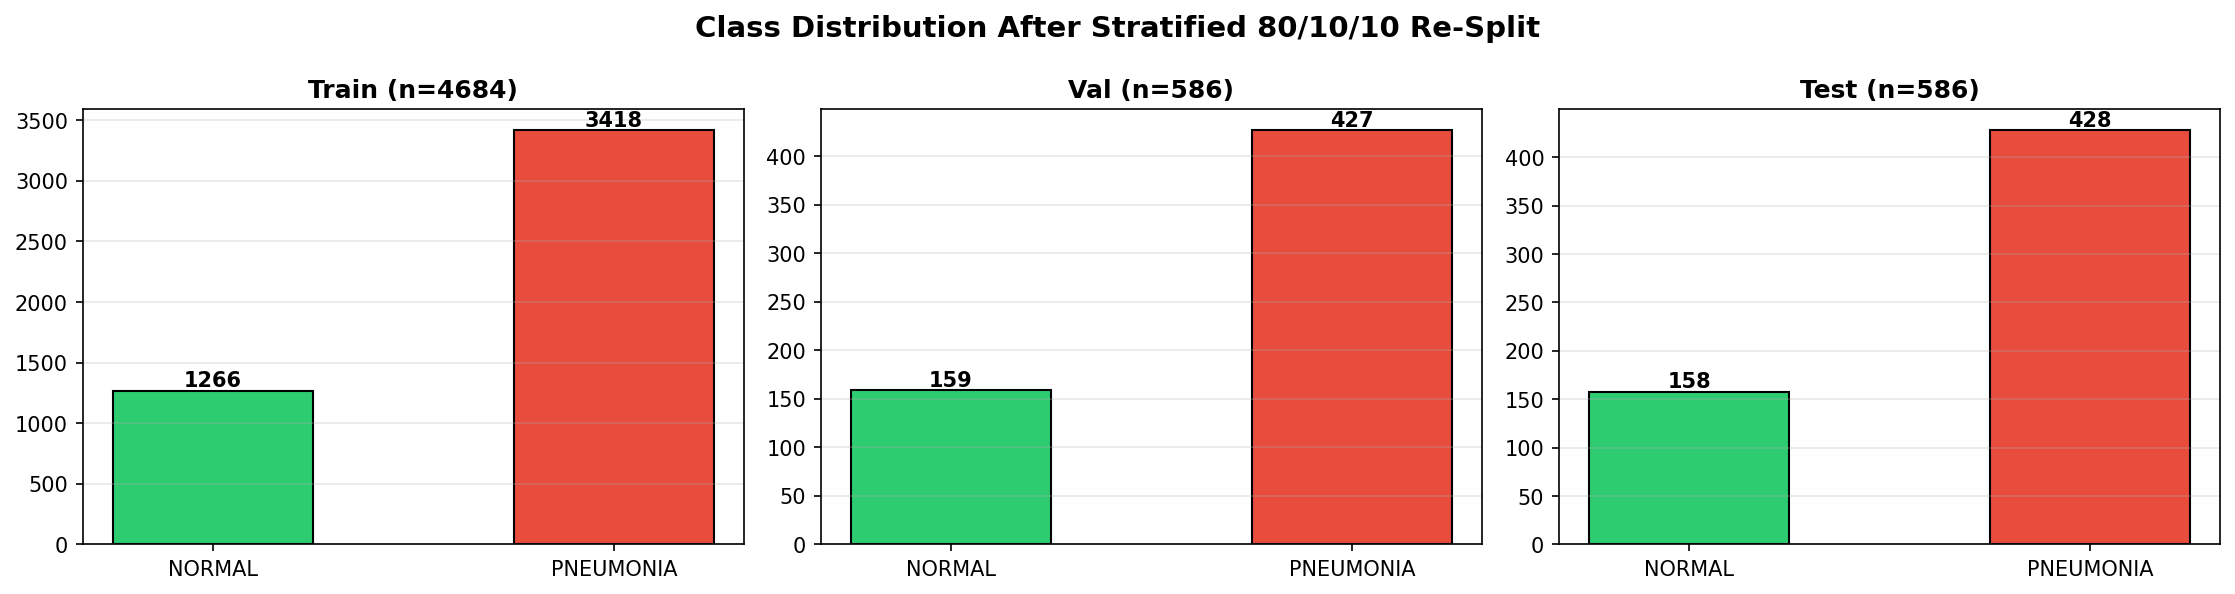
\includegraphics[width=0.7\textwidth]{p2_class_distribution.png}
\caption{Class distribution across the three partitions after stratified re-splitting.}
\label{fig:1}
\end{figure}

Figure~\ref{fig:1} shows that the $\sim$2.7:1 ratio is preserved in every split, confirming that
stratification succeeded and that test metrics are not distorted by a skewed partition.

\begin{figure}[H]
\centering
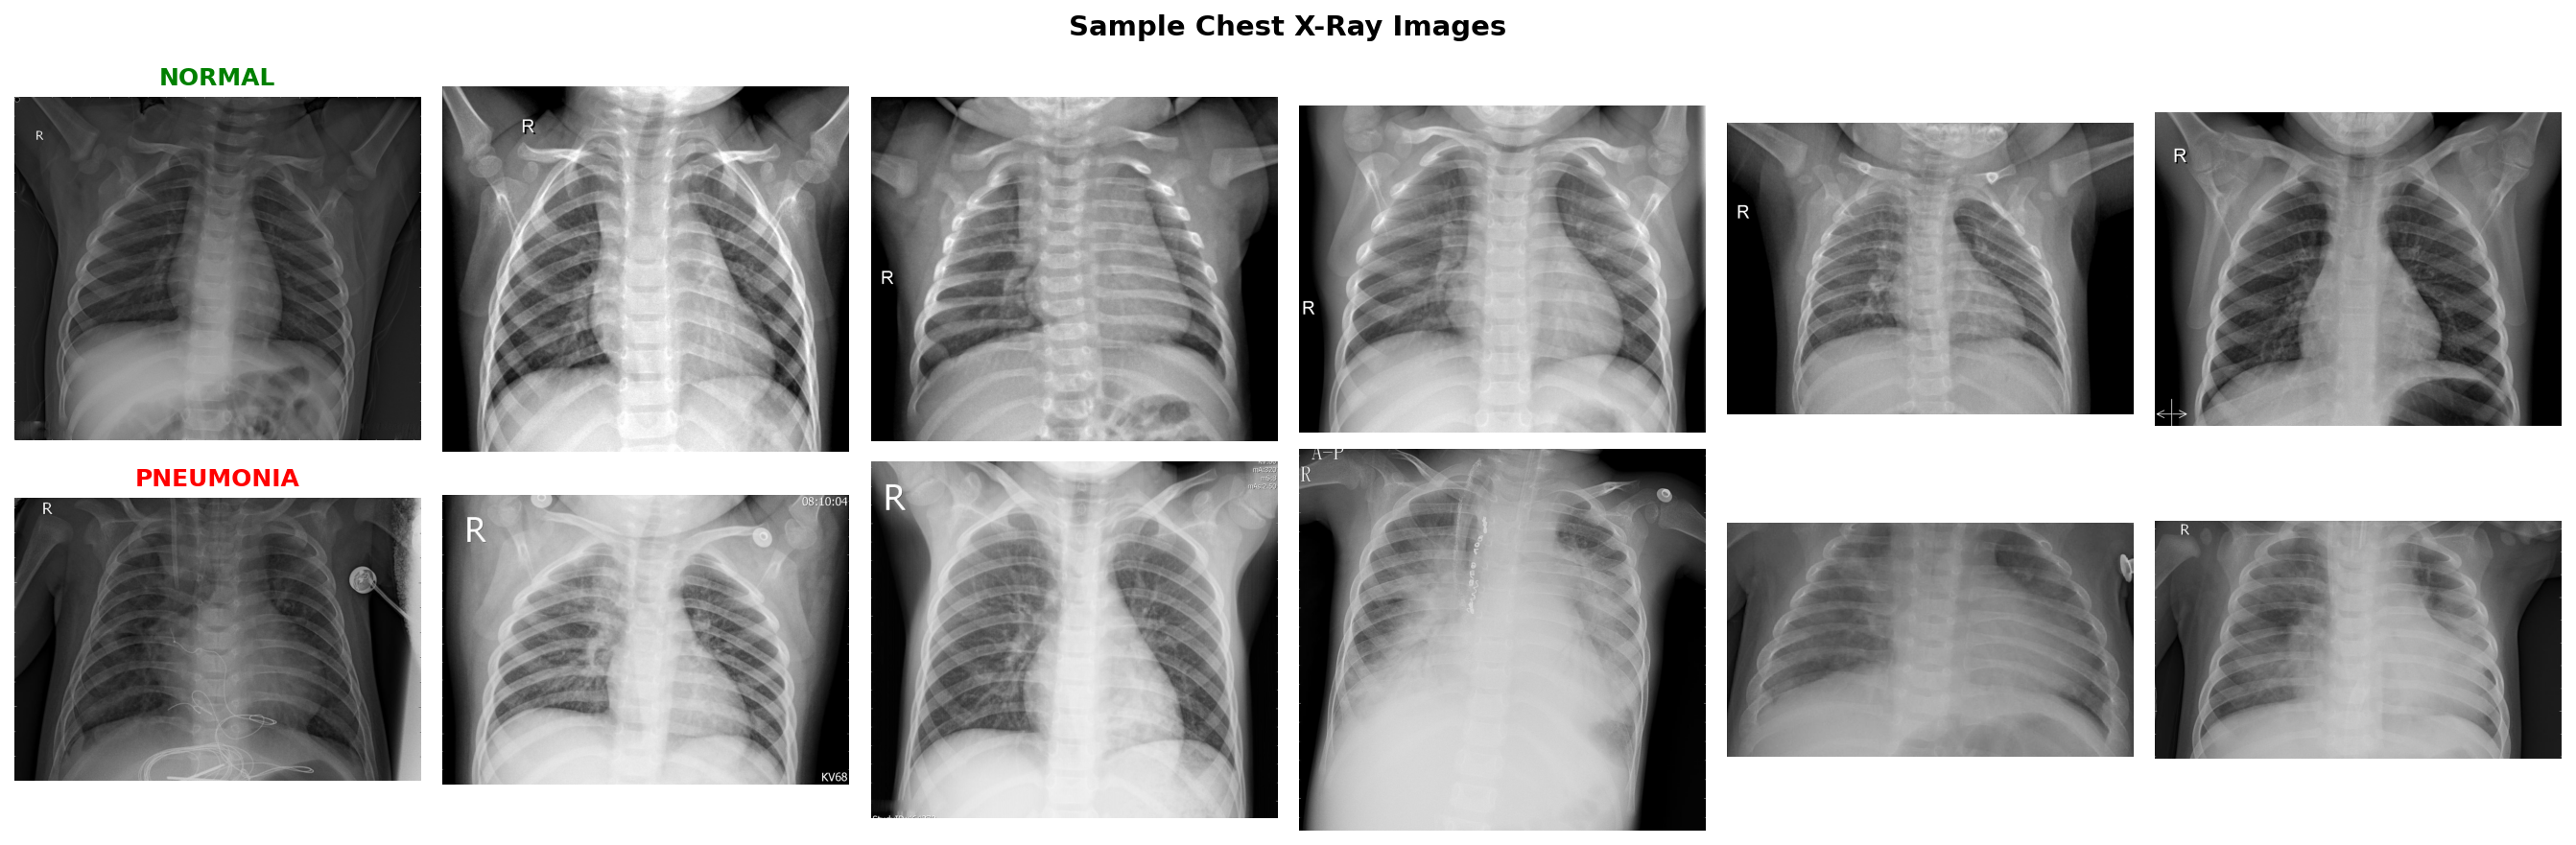
\includegraphics[width=0.8\textwidth]{p1_sample_images.png}
\caption{Representative NORMAL (top row) and PNEUMONIA (bottom row) radiographs.}
\label{fig:2}
\end{figure}

As Figure~\ref{fig:2} illustrates, normal lungs present clear fields with sharp rib and vascular detail,
whereas pneumonia presents diffuse white opacities (consolidation) obscuring the lung fields the
discriminative signal the network must learn.

All images are resized to $224\times224$, converted to three-channel RGB, and normalised using ImageNet
channel statistics (mean $=[0.485,0.456,0.406]$; std $=[0.229,0.224,0.225]$) so that pretrained weights
receive their expected input distribution. Training data are augmented with random horizontal flip
($p=0.5$), random rotation ($\pm10^\circ$), colour jitter (brightness and contrast 0.2), and small
affine translation ($\pm5\%$); validation and test data are not augmented.

Class imbalance in the corrected regime is handled by a \texttt{WeightedRandomSampler} that assigns each
training example a weight inversely proportional to its class frequency, so that each mini-batch is
approximately balanced (Section~\ref{sec:imbalance}).

\begin{figure}[H]
\centering
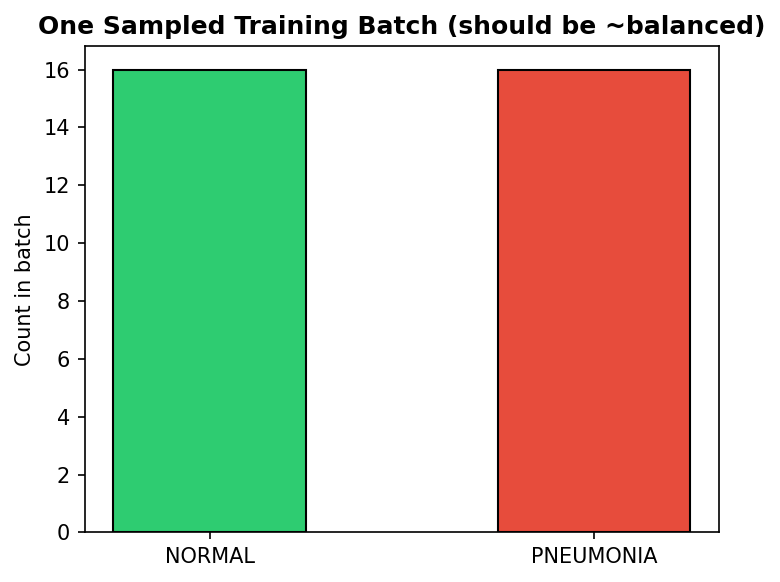
\includegraphics[width=0.7\textwidth]{p2_sampled_batch.png}
\caption{One mini-batch drawn through the weighted sampler.}
\label{fig:3}
\end{figure}

Figure~\ref{fig:3} contains 16 NORMAL and 16 PNEUMONIA examples despite the 2.7:1 dataset imbalance,
confirming that the sampler rebalances the training stream at the batch level.

% ===================================================================
\section{Methodology}

The study follows a three-stage protocol in which each experiment isolates one obstacle and the next
builds on the previous result. Figure~\ref{fig:method} gives the overview before the components are
detailed.

\begin{figure}[H]
\centering
\resizebox{\textwidth}{!}{%
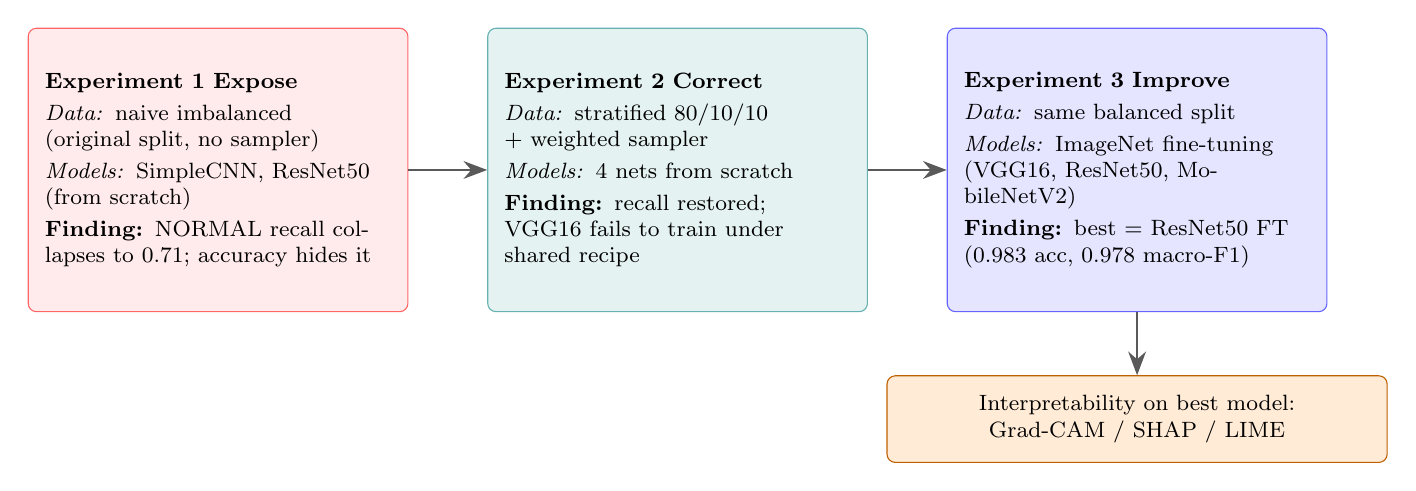
\begin{tikzpicture}[
  stage/.style={rectangle, rounded corners=3pt, align=left, font=\footnotesize,
    text width=44mm, minimum height=36mm, inner sep=6pt},
  sA/.style={stage, draw=red!60, fill=red!8},
  sB/.style={stage, draw=teal!60, fill=teal!10},
  sC/.style={stage, draw=blue!60, fill=blue!10},
  sD/.style={rectangle, rounded corners=3pt, align=center, font=\footnotesize,
    text width=60mm, minimum height=11mm, inner sep=5pt, draw=orange!75!black, fill=orange!16},
  big/.style={-{Stealth[length=3mm]}, draw=black!65, line width=1pt}]
\node[sA] (e1) {\textbf{Experiment 1   Expose}\\[2pt]
  \textit{Data:} naive imbalanced\\(original split, no sampler)\\[2pt]
  \textit{Models:} SimpleCNN, ResNet50\\(from scratch)\\[2pt]
  \textbf{Finding:} NORMAL recall collapses to 0.71; accuracy hides it};
\node[sB, right=10mm of e1] (e2) {\textbf{Experiment 2   Correct}\\[2pt]
  \textit{Data:} stratified 80/10/10\\+ weighted sampler\\[2pt]
  \textit{Models:} 4 nets from scratch\\[2pt]
  \textbf{Finding:} recall restored; VGG16 fails to train under shared recipe};
\node[sC, right=10mm of e2] (e3) {\textbf{Experiment 3   Improve}\\[2pt]
  \textit{Data:} same balanced split\\[2pt]
  \textit{Models:} ImageNet fine-tuning\\(VGG16, ResNet50, MobileNetV2)\\[2pt]
  \textbf{Finding:} best = ResNet50 FT (0.983 acc, 0.978 macro-F1)};
\node[sD, below=8mm of e3] (xai) {Interpretability on best model:\\Grad-CAM / SHAP / LIME};
\draw[big] (e1)--(e2);
\draw[big] (e2)--(e3);
\draw[big] (e3)--(xai);
\end{tikzpicture}}
\caption{Three-stage methodology: expose, correct, improve.}
\label{fig:method}
\end{figure}

Each stage reuses the data, augmentation, sampler, batch size, and optimiser family of the next so that
the change introduced at each step is the variable under study. The remainder of this section details the
architectures, the imbalance handling, and the two-phase fine-tuning procedure.

\subsection{Architectures}
Four CNNs spanning roughly a 550-fold range in parameter count are employed across the study
(Table~\ref{tab:arch}). SimpleCNN is a deliberately small, hand-built control used only in the
from-scratch experiments; the remaining three serve as both from-scratch baselines and fine-tuning
targets.

\begin{table}[H]
\centering
\caption{Architectures and their role in the study.}
\label{tab:arch}
\begin{tabularx}{\textwidth}{lrlX}
\toprule
Architecture & Parameters & Role & Rationale \\
\midrule
SimpleCNN & 0.24\,M & Scratch only & Four-block convolutional control; a weak reference point \\
MobileNetV2 \cite{mobilenet} & 2.23\,M & Scratch + fine-tune & Efficient depthwise-separable mobile network \\
ResNet50 \cite{resnet} & 23.5\,M & Scratch + fine-tune & Deep residual/bottleneck network of high capacity \\
VGG16 \cite{vgg} & 134.3\,M & Scratch + fine-tune & Large plain convolutional network \textbf{without BatchNorm} the difficult case \\
\bottomrule
\end{tabularx}
\end{table}

For fine-tuning, the classifier head of each network is adapted to the two-class problem. ResNet50 and
MobileNetV2 receive \texttt{Dropout(0.4)$\rightarrow$Linear(in\_features,\,2)}; VGG16 retains its
ImageNet 4096--4096 fully-connected stack and replaces only the final layer. Pretrained weights are
\texttt{IMAGENET1K\_V2} for ResNet50 and MobileNetV2 and \texttt{V1} for VGG16.

\begin{figure}[H]
\centering
\resizebox{\textwidth}{!}{%
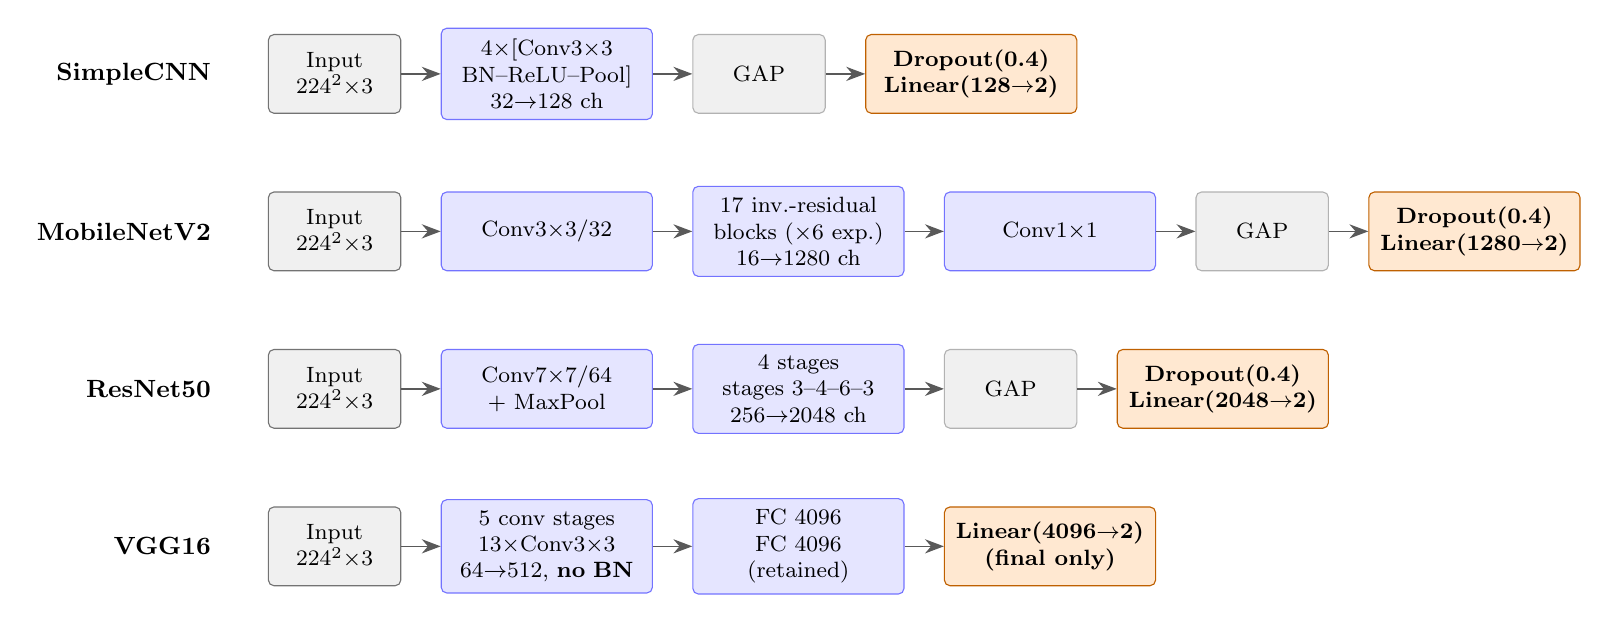
\begin{tikzpicture}[node distance=5mm and 5mm]
% ---- SimpleCNN ----
\node[io] (s_in) at (0,0) {Input\\224\textsuperscript{2}$\times$3};
\node[bbone, right=of s_in] (s_b) {4$\times$[Conv3$\times$3\\BN--ReLU--Pool]\\32\arr128 ch};
\node[pool, right=of s_b] (s_p) {GAP};
\node[head, right=of s_p] (s_h) {Dropout(0.4)\\Linear(128\arr2)};
\node[rowlbl, left=6mm of s_in] {SimpleCNN};
\draw[flow] (s_in)--(s_b); \draw[flow] (s_b)--(s_p); \draw[flow] (s_p)--(s_h);
% ---- MobileNetV2 ----
\node[io] (m_in) at (0,-2.0) {Input\\224\textsuperscript{2}$\times$3};
\node[bbone, right=of m_in] (m_b1) {Conv3$\times$3/32};
\node[bbone, right=of m_b1] (m_b2) {17 inv.-residual\\blocks ($\times6$ exp.)\\16\arr1280 ch};
\node[bbone, right=of m_b2] (m_b3) {Conv1$\times$1};
\node[pool, right=of m_b3] (m_p) {GAP};
\node[head, right=of m_p] (m_h) {Dropout(0.4)\\Linear(1280\arr2)};
\node[rowlbl, left=6mm of m_in] {MobileNetV2};
\draw[flow] (m_in)--(m_b1); \draw[flow] (m_b1)--(m_b2); \draw[flow] (m_b2)--(m_b3);
\draw[flow] (m_b3)--(m_p); \draw[flow] (m_p)--(m_h);
% ---- ResNet50 ----
\node[io] (r_in) at (0,-4.0) {Input\\224\textsuperscript{2}$\times$3};
\node[bbone, right=of r_in] (r_b1) {Conv7$\times$7/64\\+ MaxPool};
\node[bbone, right=of r_b1] (r_b2) {4 stages\\stages 3--4--6--3\\256\arr2048 ch};
\node[pool, right=of r_b2] (r_p) {GAP};
\node[head, right=of r_p] (r_h) {Dropout(0.4)\\Linear(2048\arr2)};
\node[rowlbl, left=6mm of r_in] {ResNet50};
\draw[flow] (r_in)--(r_b1); \draw[flow] (r_b1)--(r_b2); \draw[flow] (r_b2)--(r_p); \draw[flow] (r_p)--(r_h);
% ---- VGG16 ----
\node[io] (v_in) at (0,-6.0) {Input\\224\textsuperscript{2}$\times$3};
\node[bbone, right=of v_in] (v_b1) {5 conv stages\\13$\times$Conv3$\times$3\\64\arr512, \textbf{no BN}};
\node[bbone, right=of v_b1] (v_b2) {FC 4096\\FC 4096\\(retained)};
\node[head, right=of v_b2] (v_h) {Linear(4096\arr2)\\(final only)};
\node[rowlbl, left=6mm of v_in] {VGG16};
\draw[flow] (v_in)--(v_b1); \draw[flow] (v_b1)--(v_b2); \draw[flow] (v_b2)--(v_h);
\end{tikzpicture}}
\caption{Architecture specifications: backbone (reused) to replaced classifier head.}
\label{fig:arch2}
\end{figure}

Each network in Figure~\ref{fig:arch2} accepts a $224\times224\times3$ input and emits two logits.
\textcolor{blue!55}{\textbf{Blue}} marks the ImageNet-pretrained backbone (reused),
\textcolor{gray!70}{\textbf{grey}} the global average pooling, and
\textcolor{orange!75!black}{\textbf{orange}} the classifier head replaced for the two-class task. VGG16
retains its 4096--4096 fully-connected stack and replaces only the final layer.

A block-level diagram for ResNet50 (the best model) can be regenerated from the trained network with
\texttt{torchview.draw\_graph(model, input\_size=(1,3,224,224))}; the schematic flow is
\texttt{Input 224\textsuperscript{2} $\rightarrow$ conv/pool stem $\rightarrow$ [stage1$\times$3
$\rightarrow$ stage2$\times$4 $\rightarrow$ stage3$\times$6 $\rightarrow$ stage4$\times$3] residual
bottlenecks $\rightarrow$ GAP $\rightarrow$ Dropout $\rightarrow$ Linear(2048$\rightarrow$2) $\rightarrow$
softmax}.

\subsection{Rationale for transfer learning}
Training a deep CNN from random initialisation requires a large and diverse dataset to learn the full
visual feature hierarchy. The training partition here contains only 4{,}684 images. A network pretrained
on ImageNet \cite{imagenet} already encodes reusable low- and mid-level features; although chest
radiographs are grayscale and out-of-domain, these early features are largely domain-agnostic and
transfer effectively. The clearest empirical confirmation in this study is VGG16, which fails to optimise
from scratch under our shared, architecture-agnostic recipe (the single learning rate of
$1\mathrm{e}{-3}$ applied to every from-scratch model) yet becomes competitive once fine-tuned
(Section~\ref{sec:results}). We are careful not to claim that VGG16 is intrinsically untrainable from
random initialisation with VGG-specific tuning (a smaller learning rate and warm-up) it can be trained,
as in the original work; the point is that fine-tuning proved robust to the very recipe under which
from-scratch VGG16 collapsed.

\subsection{Class-imbalance handling: weighted random sampling}
\label{sec:imbalance}
The assignment permits either class-weighted loss or oversampling; oversampling at the batch level was
selected. Each training sample receives a weight inversely proportional to its class frequency, so that
minority (NORMAL) examples are drawn more often:

\begin{lstlisting}
class_count  = Counter(train_labels)        # {1: 3418, 0: 1266}
class_w      = {c: 1.0 / n for c, n in class_count.items()}
sample_w     = [class_w[t] for t in train_labels]
sampler      = WeightedRandomSampler(sample_w,
                 num_samples=len(sample_w), replacement=True)
train_loader = DataLoader(train_dataset, batch_size=32,
                 sampler=sampler, ...)
\end{lstlisting}

With sampling performed with replacement, minority images may recur within an epoch, yielding
approximately class-balanced mini-batches (Figure~\ref{fig:3}) and gradient updates that are not
dominated by the majority class. The validation and test loaders use no sampler, so all reported metrics
reflect the true class distribution. Oversampling was preferred over class-weighted loss because it
rebalances the data stream directly, leaving the loss surface and label-smoothing behaviour unmodified.

\subsection{Two-phase fine-tuning, matched to architecture}
\label{sec:finetune}
Unfreezing an entire pretrained network at a high learning rate destroys its features: large gradients
originating from the randomly-initialised head propagate into the backbone and overwrite the pretrained
weights. Fine-tuning is therefore performed in two phases, and importantly the Phase-2 unfreezing
scope is matched to each architecture.
\begin{itemize}
\item \textbf{Phase 1 (head warm-up).} The backbone is frozen and only the new head is trained.
BatchNorm \cite{batchnorm} running statistics are held fixed (\texttt{model.apply(set\_bn\_eval)}) so
that the frozen backbone does not drift from its ImageNet calibration. Targets are softened with label
smoothing.
\item \textbf{Phase 2 (controlled unfreeze).} Layers are unfrozen and trained with discriminative
learning rates, the head faster than the backbone.
\end{itemize}

\begin{table}[H]
\centering
\caption{Per-architecture fine-tuning configuration.}
\label{tab:ftcfg}
\small
\begin{tabularx}{\textwidth}{
    >{\raggedright\arraybackslash}p{2.5cm}
    >{\raggedright\arraybackslash}p{4cm}
    >{\raggedright\arraybackslash}p{3.2cm}
    >{\centering\arraybackslash}p{2.2cm}
    >{\raggedright\arraybackslash}X
}
\toprule
Backbone & Phase 1 & Phase 2 unfreeze & Head/backbone LR & Stabilisers \\
\midrule
VGG16 (no BN, 134\,M) & head warm-up, 6 ep, LR 5e-4, BN frozen & last conv block only (94\% trainable) & 1e-4 / \textbf{1e-5} & grad clip 2.0, LS 0.05 \\
ResNet50 (BN + residual) & head only, 5 ep, LR 1e-3, BN frozen & \textbf{full} (100\%) & 3e-4 / 1e-4 & LS 0.1 \\
MobileNetV2 (BN, light) & head only, 5 ep, LR 1e-3, BN frozen & \textbf{full} (100\%) & 3e-4 / 1e-4 & LS 0.1 \\
\bottomrule
\end{tabularx}
\end{table}

VGG16, lacking BatchNorm and carrying 134\,M parameters, is the fragile case: a full unfreeze would
destabilise its convolutional filters, so it receives the gentlest treatment partial unfreeze, a very
small backbone learning rate, and gradient clipping. ResNet50 and MobileNetV2 are stabilised by
BatchNorm and tolerate a full unfreeze. The Phase-2 optimiser uses parameter groups:

\begin{lstlisting}
optimizer = optim.Adam([
    {'params': backbone_params, 'lr': lr_backbone}, # gentle
    {'params': head_params,     'lr': lr},          # faster
])
\end{lstlisting}

The from-scratch controls omit this procedure entirely: random initialisation, all layers trainable from
the first epoch, and a single learning rate of $1\mathrm{e}{-3}$. Data, augmentation, sampler, batch
size, and optimiser family are held constant across both paths. Pretraining is therefore the
\textbf{primary} distinguishing variable, but it is not the only one: the fine-tuning path additionally
introduces label smoothing, a two-phase schedule with discriminative learning rates, and test-time
augmentation at evaluation (Section~\ref{sec:threats}). The scratch--fine-tune deltas in
Table~\ref{tab:delta} should accordingly be read as the combined effect of the full transfer-learning
protocol rather than of pretraining in isolation; the direction and magnitude of the VGG16 result,
however, are too large to be attributable to these auxiliary factors alone.

\subsection{Shared training configuration}
\begin{table}[H]
\centering
\caption{Shared hyperparameters.}
\label{tab:hyper}
\begin{tabularx}{\textwidth}{lX}
\toprule
Hyperparameter & Value \\
\midrule
Optimiser & Adam \\
LR scheduler & ReduceLROnPlateau (factor 0.5, patience 3, on validation loss) \\
Batch size & 32 \\
Loss & Cross-entropy (label smoothing 0.05--0.1 for fine-tuning) \\
Epoch budget & 20 (Exp.\ 1); 25 (Exp.\ 2); 5--6 + 15--20 two-phase (Exp.\ 3) \\
Early stopping & patience 6--7 epochs \\
Checkpoint criterion & maximum (validation accuracy + validation AUC), ties broken by lower validation loss \\
Test-time augmentation & mean of original and horizontally-flipped predictions (Exp.\ 3) \\
Random seed & 42 (PyTorch and NumPy) \\
Hardware / framework & CUDA GPU, PyTorch 2.10 \cite{pytorch} \\
\bottomrule
\end{tabularx}
\end{table}

\subsection{Training pipeline}
\begin{figure}[H]
\centering
\resizebox{0.92\textwidth}{!}{%
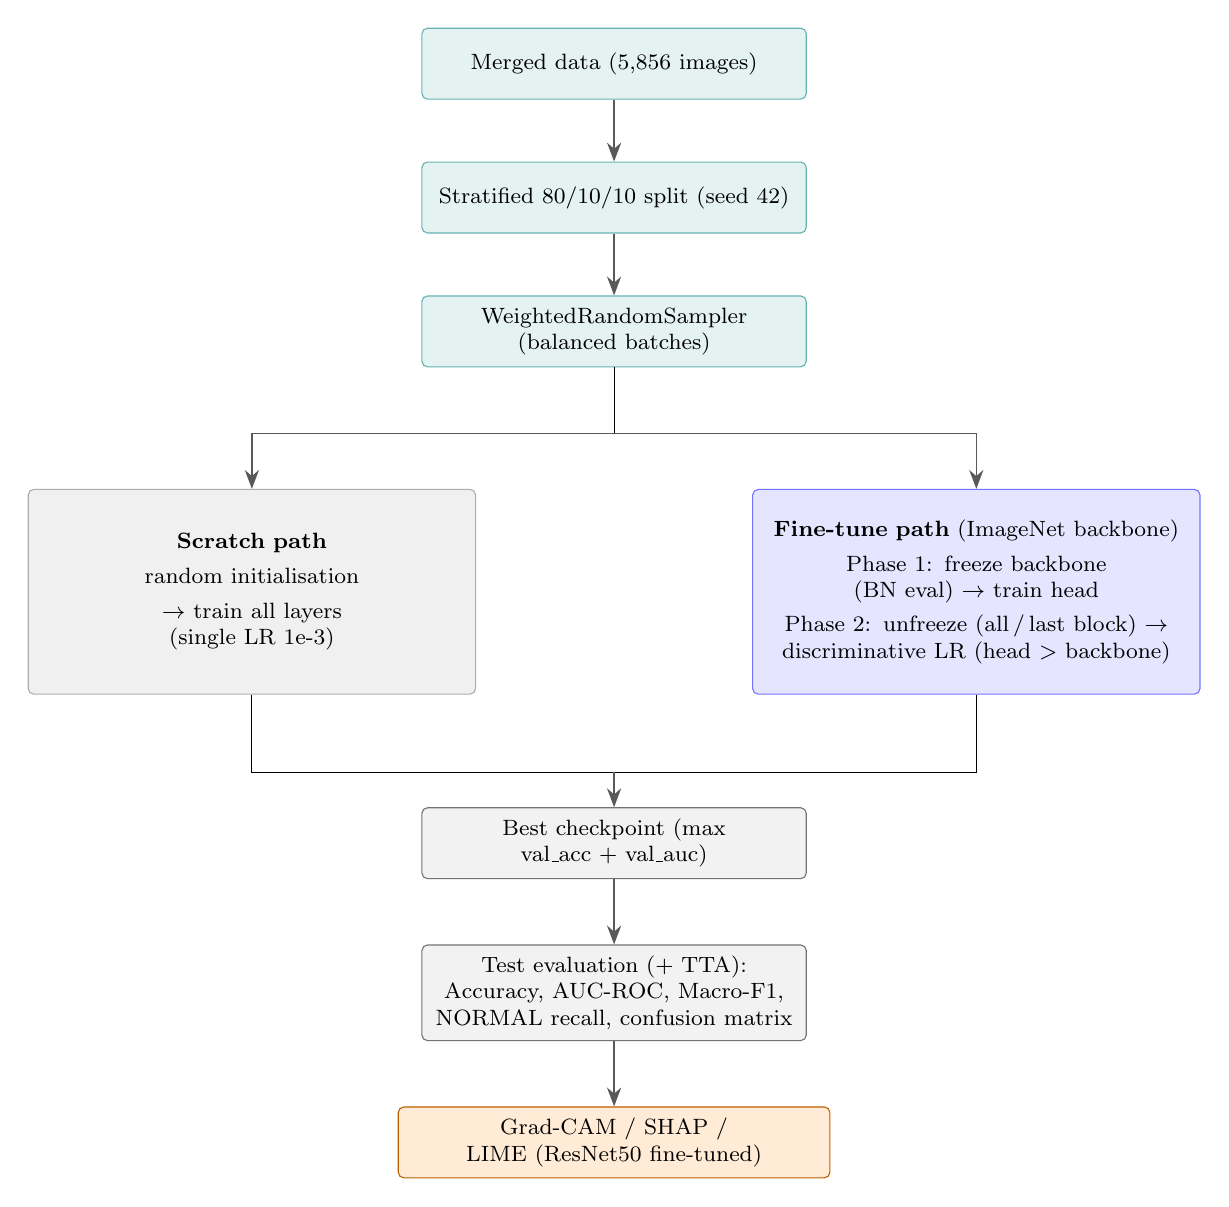
\begin{tikzpicture}[every node/.style={font=\footnotesize}]
% ---- data-prep spine ----
\node[fdata] (n1) at (0,0) {Merged data (5{,}856 images)};
\node[fdata] (n2) at (0,-1.7) {Stratified 80/10/10 split (seed 42)};
\node[fdata] (n3) at (0,-3.4) {WeightedRandomSampler (balanced batches)};
% ---- split junction ----
\coordinate (split) at (0,-4.7);
% ---- two training paths (equal height, tops aligned) ----
\node[fscr, text width=54mm, minimum height=26mm, anchor=north] (scr)
  at (-4.6,-5.4) {\textbf{Scratch path}\\[3pt] random initialisation\\[3pt]
  \arr{} train all layers\\(single LR 1e-3)};
\node[fft, text width=54mm, minimum height=26mm, anchor=north] (ft)
  at (4.6,-5.4) {\textbf{Fine-tune path} (ImageNet backbone)\\[3pt]
  Phase 1: freeze backbone (BN eval) \arr{} train head\\[3pt]
  Phase 2: unfreeze (all\,/\,last block) \arr{} discriminative LR (head $>$ backbone)};
% ---- merge junction ----
\coordinate (merge) at (0,-9.0);
% ---- evaluation spine ----
\node[fstep] (cp)   at (0,-9.9) {Best checkpoint (max val\_acc + val\_auc)};
\node[fstep] (eval) at (0,-11.8) {Test evaluation (+ TTA):\\Accuracy, AUC-ROC, Macro-F1, NORMAL recall, confusion matrix};
\node[fout]  (xai)  at (0,-13.7) {Grad-CAM / SHAP / LIME (ResNet50 fine-tuned)};
% ---- arrows ----
\draw[flow] (n1) -- (n2);
\draw[flow] (n2) -- (n3);
% spine down to split, then branch with right-angle elbows
\draw (n3.south) -- (split);
\draw[flow] (split) -| (scr.north);
\draw[flow] (split) -| (ft.north);
% paths down, merge with right-angle elbows into the spine
\draw (scr.south) |- (merge);
\draw (ft.south)  |- (merge);
\draw[flow] (merge) -- (cp.north);
\draw[flow] (cp) -- (eval);
\draw[flow] (eval) -- (xai);
\end{tikzpicture}}
\caption{End-to-end training pipeline.}
\label{fig:pipeline}
\end{figure}

In Figure~\ref{fig:pipeline}, \textcolor{teal!70}{\textbf{teal}} marks data preparation,
\textcolor{gray!70}{\textbf{grey}} the from-scratch path, \textcolor{blue!55}{\textbf{blue}} the
two-phase fine-tuning path, and \textcolor{orange!75!black}{\textbf{orange}} interpretability on the best
model. Both training paths share data, augmentation, sampler, batch size, and optimiser family;
pretraining (plus the auxiliary fine-tuning protocol) is the distinguishing variable.

% ===================================================================
\section{Results}
\label{sec:results}

\subsection{Experiment 1: Naive imbalanced baseline}
Two networks were trained from scratch on the original imbalanced partition using plain cross-entropy
with no sampler. The test set comprises 624 images (234 NORMAL, 390 PNEUMONIA).

\begin{table}[H]
\centering
\caption{Imbalanced baseline (Experiment 1).}
\label{tab:exp1}
\setlength{\tabcolsep}{4pt}
% column widths (mm): Model 30 | Acc 17 | AUC 17 | NORMALrec 20 | PNEUMONIArec 24 | F1 17
\begin{tabular}{L{30mm} C{17mm} C{17mm} C{20mm} C{24mm} C{17mm}}
\toprule
Model & Accuracy & AUC-ROC & NORMAL recall & PNEUMONIA recall & Macro-F1 \\
\midrule
SimpleCNN (imbalanced) & 0.8718 & 0.9254 & 0.8547 & 0.8821 & 0.8646 \\
ResNet50 (imbalanced) & 0.8670 & 0.9480 & \textbf{0.7051} & 0.9641 & 0.8498 \\
\bottomrule
\end{tabular}
\end{table}

The central observation is that ResNet50 reports a plausible overall accuracy (86.7\%) while its NORMAL
recall falls to 0.71: roughly three in ten healthy patients are misclassified as having pneumonia, driven
by the network's bias toward the majority class. Accuracy alone conceals this behaviour, which motivates
reporting per-class recall and AUC-ROC throughout.

\begin{figure}[H]
\centering
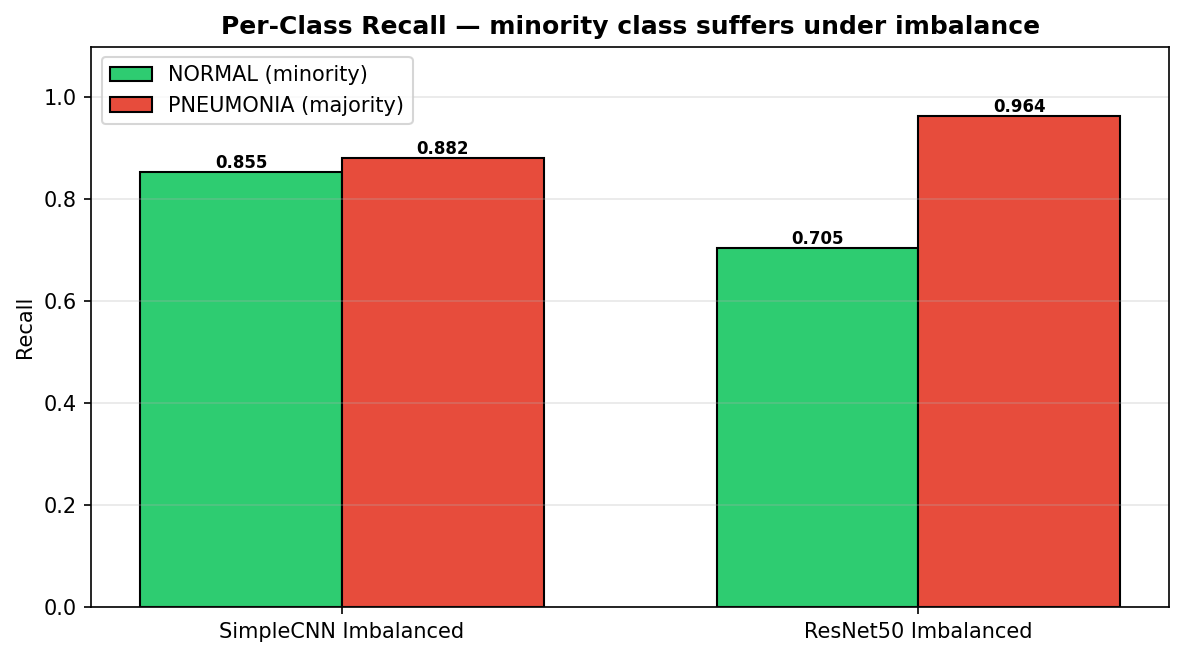
\includegraphics[width=0.7\textwidth]{p1_per_class_recall.png}
\caption{Per-class recall under imbalance.}
\label{fig:4}
\end{figure}

Figure~\ref{fig:4} shows the collapse of ResNet50's minority (NORMAL) recall relative to its majority
recall the failure that overall accuracy hides.

\begin{figure}[H]
\centering
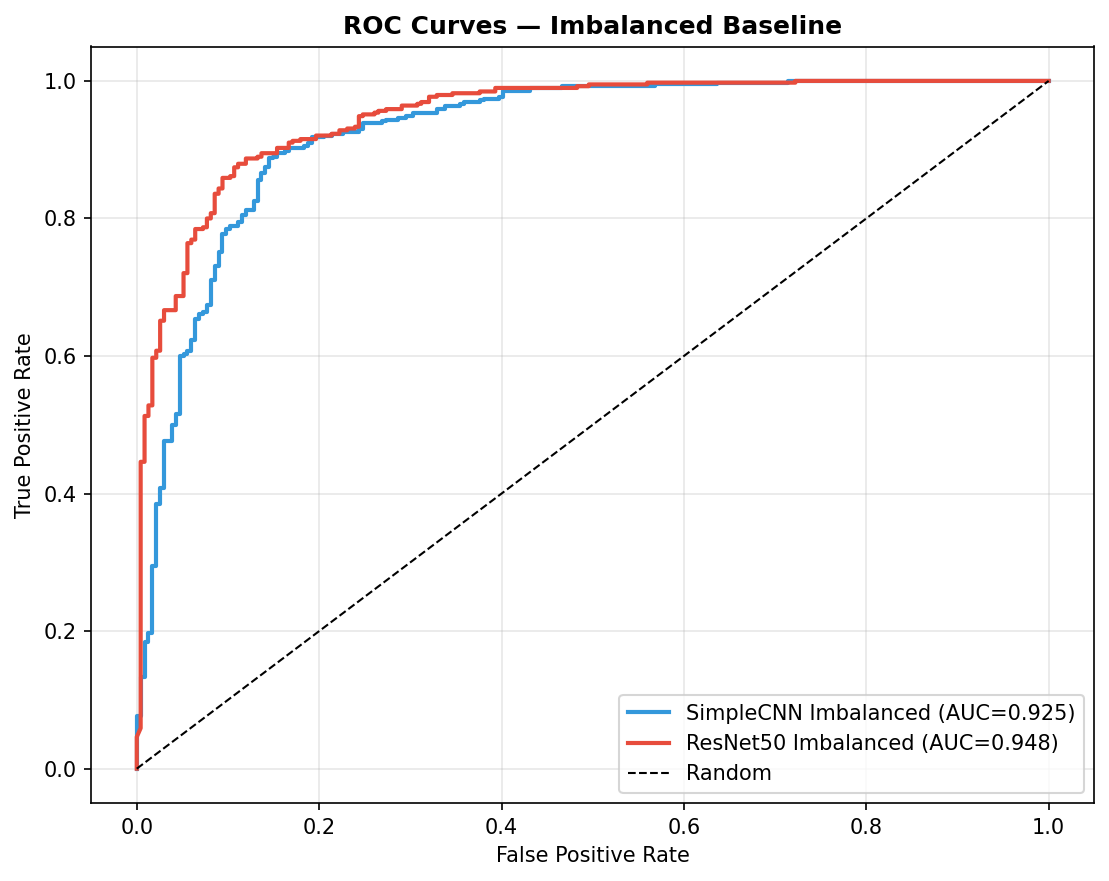
\includegraphics[width=0.7\textwidth]{p1_roc_curves.png}
\caption{ROC curves for the imbalanced baseline.}
\label{fig:5}
\end{figure}

In Figure~\ref{fig:5}, ranking quality (AUC) remains moderate even though the operating-point recall on
the minority class is poor, illustrating why threshold-dependent and threshold-independent metrics must
be read together.

\subsection{Experiment 2: Balanced from-scratch baselines}
Using the corrected regime (stratified split and weighted sampler), four randomly-initialised networks
were trained. The test set comprises 586 images.

\begin{table}[H]
\centering
\caption{From-scratch (balanced) results. Bold indicates the best value per column.}
\label{tab:exp2}
\setlength{\tabcolsep}{4pt}
% column widths (mm): Model 34 | Params 20 | Acc 18 | AUC 17 | F1 17 | NORMALrec 20
\begin{tabular}{L{34mm} C{20mm} C{18mm} C{17mm} C{17mm} C{20mm}}
\toprule
Model & Parameters & Accuracy & AUC-ROC & Macro-F1 & NORMAL recall \\
\midrule
SimpleCNN (scratch) & 0.24\,M & 0.9590 & 0.9825 & 0.9462 & 0.8734 \\
VGG16 (scratch) & 134.3\,M & 0.7304 & 0.6268 & 0.4221 & 0.0000 \\
ResNet50 (scratch) & 23.5\,M & \textbf{0.9710} & \textbf{0.9963} & \textbf{0.9632} & 0.9494 \\
MobileNetV2 (scratch) & 2.23\,M & 0.9608 & 0.9955 & 0.9510 & \textbf{0.9557} \\
\bottomrule
\end{tabular}
\end{table}

Two findings stand out. First, the weighted sampler is effective: minority recall recovers relative to
Experiment~1, and accuracy and recall now move together rather than in opposition. This cross-experiment
comparison is indicative rather than exact, because Experiment~1 is evaluated on the original 624-image
test partition whereas Experiments~2 and 3 use the 586-image re-split; the two are therefore not the same
test set, and the recall figures should be read as a qualitative trend, not a paired difference. Second,
VGG16 fails to train from scratch under the shared recipe its training loss never departs from 0.693
(the random-guess value) and it predicts PNEUMONIA for every test image (0.00 NORMAL recall). Lacking
BatchNorm and carrying 134\,M parameters, VGG16 is highly sensitive to optimisation settings: at the
single learning rate ($1\mathrm{e}{-3}$) applied uniformly to all from-scratch models it does not
converge. This does not establish that VGG16 is intrinsically untrainable from random
initialisation with architecture-specific tuning (a smaller learning rate and warm-up) it can be
trained, as in the original VGG work but it shows that fine-tuning is far more robust to a fixed,
architecture-agnostic recipe, which is precisely the regime in which transfer learning is expected to
help.

\begin{figure}[H]
\centering
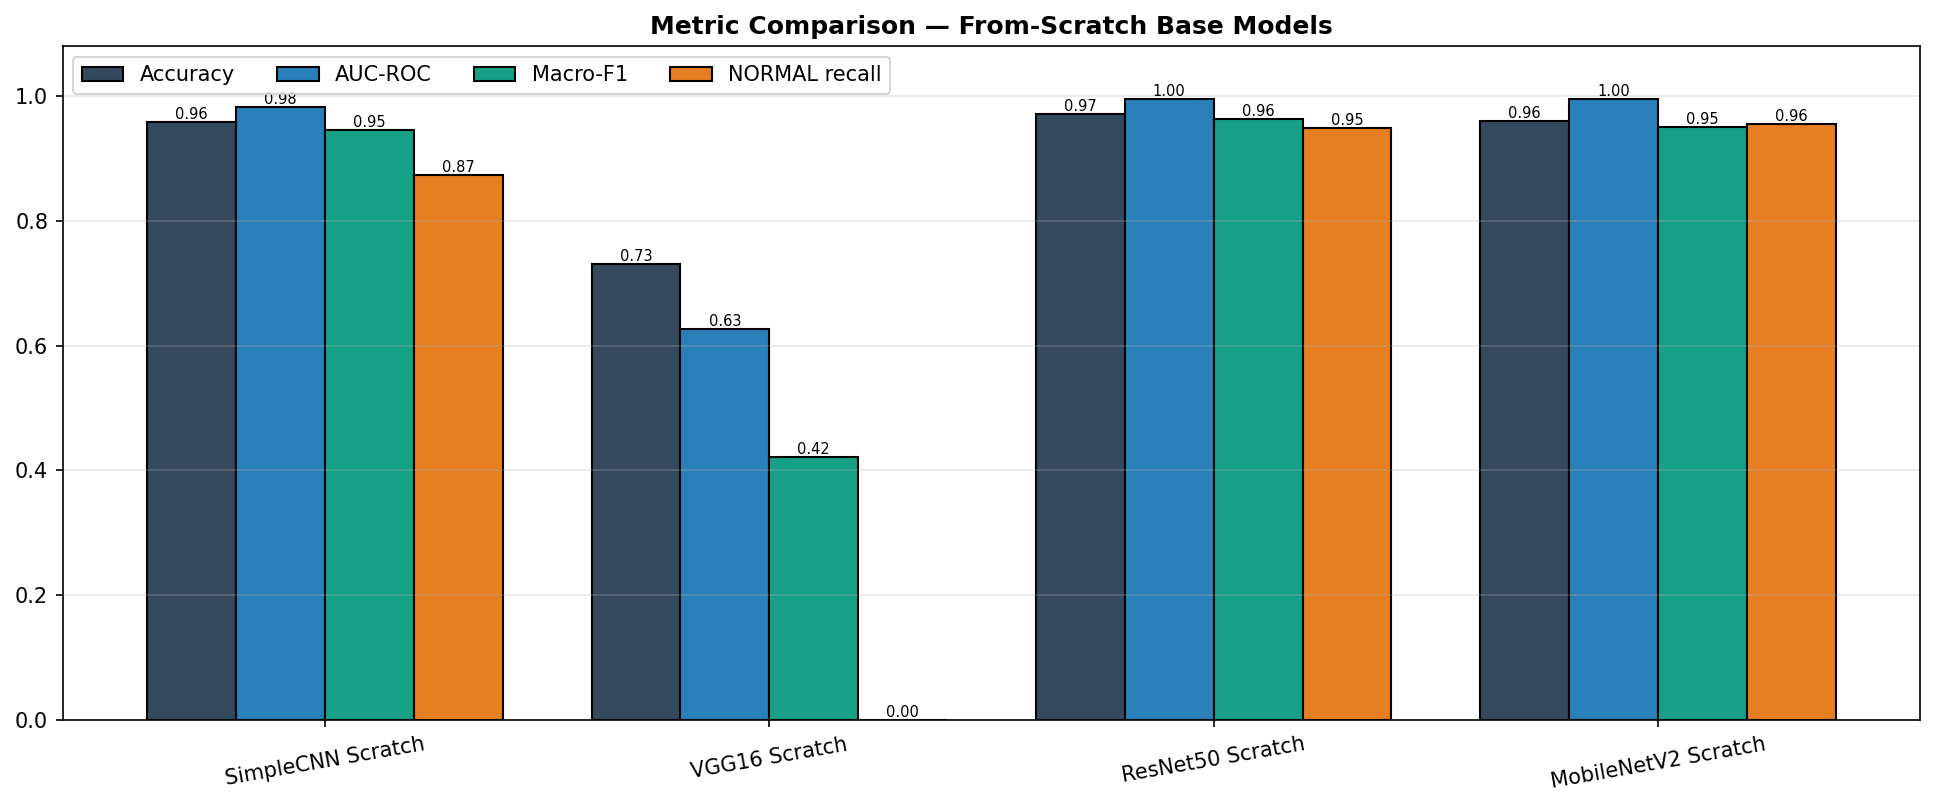
\includegraphics[width=0.8\textwidth]{p2_metric_comparison.png}
\caption{Metric comparison across the four from-scratch models.}
\label{fig:6}
\end{figure}

In Figure~\ref{fig:6} the collapse of VGG16 is visible on every metric, while the remaining three cluster
near the top of the range.

\begin{figure}[H]
\centering
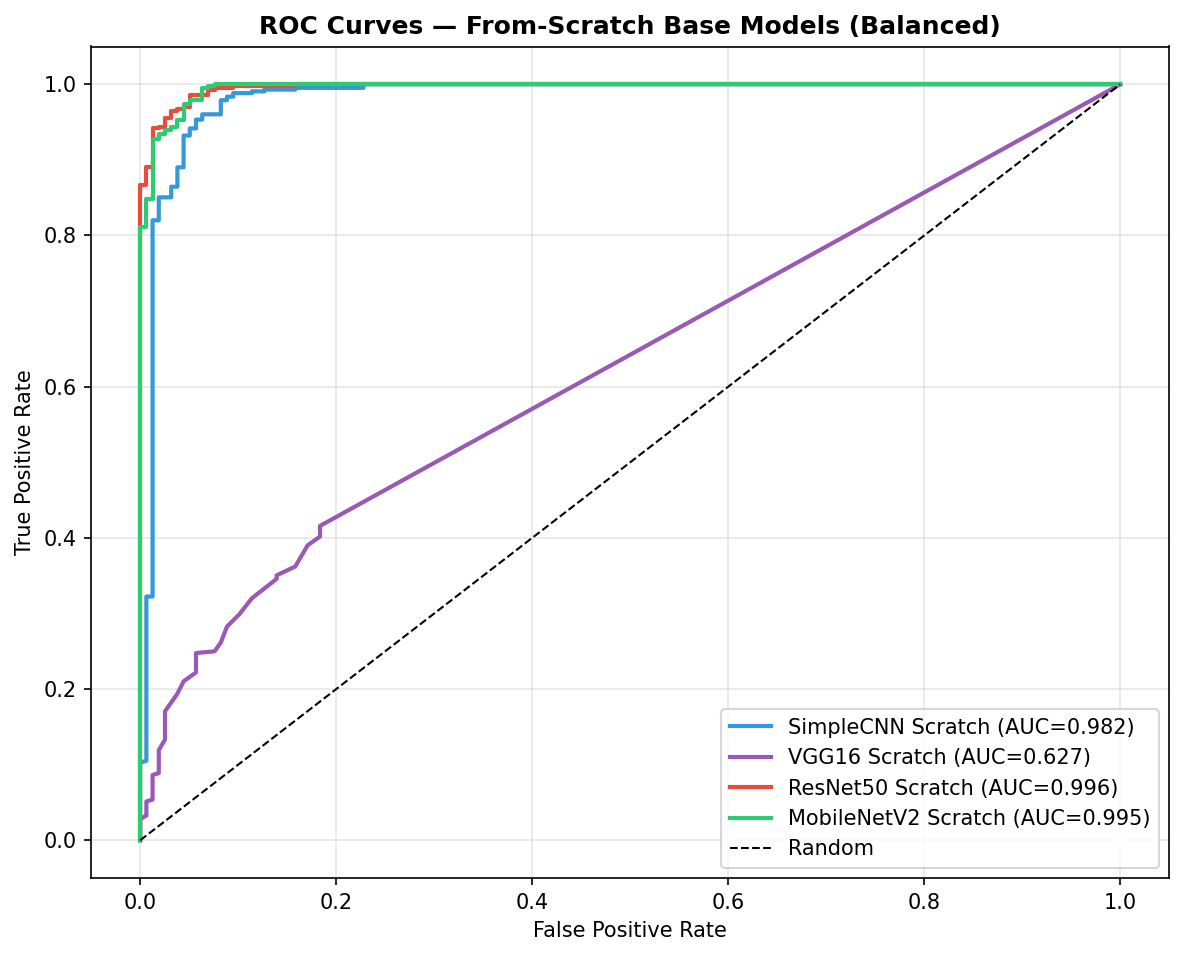
\includegraphics[width=0.7\textwidth]{p2_roc_curves.png}
\caption{ROC curves for the from-scratch models.}
\label{fig:7}
\end{figure}

In Figure~\ref{fig:7}, ResNet50 and MobileNetV2 approach the top-left corner (AUC $\approx0.996$),
whereas VGG16 lies near the diagonal (AUC 0.627).

\subsection{Experiment 3: Fine-tuned models and the scratch vs fine-tune comparison}
Three ImageNet-pretrained backbones were fine-tuned on the identical balanced split. The test set
comprises 586 images.

\begin{table}[H]
\centering
\caption{Fine-tuned results. Bold indicates the best value per column.}
\label{tab:exp3}
\setlength{\tabcolsep}{4pt}
% column widths (mm): Model 32 | Acc 17 | AUC 17 | F1 17 | NORMALrec 20 | PNEUMONIArec 24
\begin{tabular}{L{32mm} C{17mm} C{17mm} C{17mm} C{20mm} C{24mm}}
\toprule
Model & Accuracy & AUC-ROC & Macro-F1 & NORMAL recall & PNEUMONIA recall \\
\midrule
VGG16 (fine-tuned) & 0.9590 & \textbf{0.9953} & 0.9496 & 0.9747 & 0.9533 \\
ResNet50 (fine-tuned) & \textbf{0.9829} & 0.9907 & \textbf{0.9784} & 0.9747 & \textbf{0.9860} \\
MobileNetV2 (fine-tuned) & 0.9676 & 0.9944 & 0.9597 & 0.9747 & 0.9650 \\
\bottomrule
\end{tabular}
\end{table}

The best overall configuration is \textbf{ResNet50 fine-tuned} (0.9829 accuracy, 0.9784 macro-F1). All
three fine-tuned models record an identical NORMAL recall of 0.9747; this is not a transcription error
but the same count 154 of the 158 NORMAL test cases classified correctly by each model a coincidence
made possible by the small (158-image) minority test partition. Table~\ref{tab:delta} reports the
controlled comparison: each fine-tuned model against its from-scratch counterpart on four metrics.

\begin{table}[H]
\centering
\caption{Scratch $\rightarrow$ fine-tuned change, by architecture and metric.}
\label{tab:delta}
\setlength{\tabcolsep}{4pt}
% column widths (mm): Arch 26 | Metric 28 | Scratch 20 | Fine-tuned 22 | Delta 22 | Improved 18
\begin{tabular}{L{26mm} L{28mm} C{20mm} C{22mm} C{22mm} C{18mm}}
\toprule
Architecture & Metric & Scratch & Fine-tuned & $\Delta$ & Improved \\
\midrule
VGG16 & Accuracy & 0.7304 & 0.9590 & \textbf{+0.2286} & yes \\
VGG16 & AUC-ROC & 0.6268 & 0.9953 & \textbf{+0.3685} & yes \\
VGG16 & Macro-F1 & 0.4221 & 0.9496 & \textbf{+0.5275} & yes \\
VGG16 & NORMAL recall & 0.0000 & 0.9747 & \textbf{+0.9747} & yes \\
ResNet50 & Accuracy & 0.9710 & 0.9829 & +0.0119 & yes \\
ResNet50 & AUC-ROC & 0.9963 & 0.9907 & $-0.0056$ & no \\
ResNet50 & Macro-F1 & 0.9632 & 0.9784 & +0.0152 & yes \\
ResNet50 & NORMAL recall & 0.9494 & 0.9747 & +0.0253 & yes \\
MobileNetV2 & Accuracy & 0.9608 & 0.9676 & +0.0068 & yes \\
MobileNetV2 & AUC-ROC & 0.9955 & 0.9944 & $-0.0011$ & no \\
MobileNetV2 & Macro-F1 & 0.9510 & 0.9597 & +0.0087 & yes \\
MobileNetV2 & NORMAL recall & 0.9557 & 0.9747 & +0.0190 & yes \\
\bottomrule
\end{tabular}
\end{table}

\textit{Reading Table~\ref{tab:delta}.} With a single seed per configuration (Section~\ref{sec:limits})
no variance is available, so small deltas cannot be distinguished from run-to-run noise. The
``Improved'' column records only the \emph{direction} of the point estimate. Every ResNet50 and
MobileNetV2 delta has magnitude below $\approx0.025$ and should be read as ``no measurable change''
rather than as a demonstrated improvement; only the VGG16 row (deltas of $+0.23$ to $+0.97$) is large
enough to be unambiguous.

\begin{figure}[H]
\centering
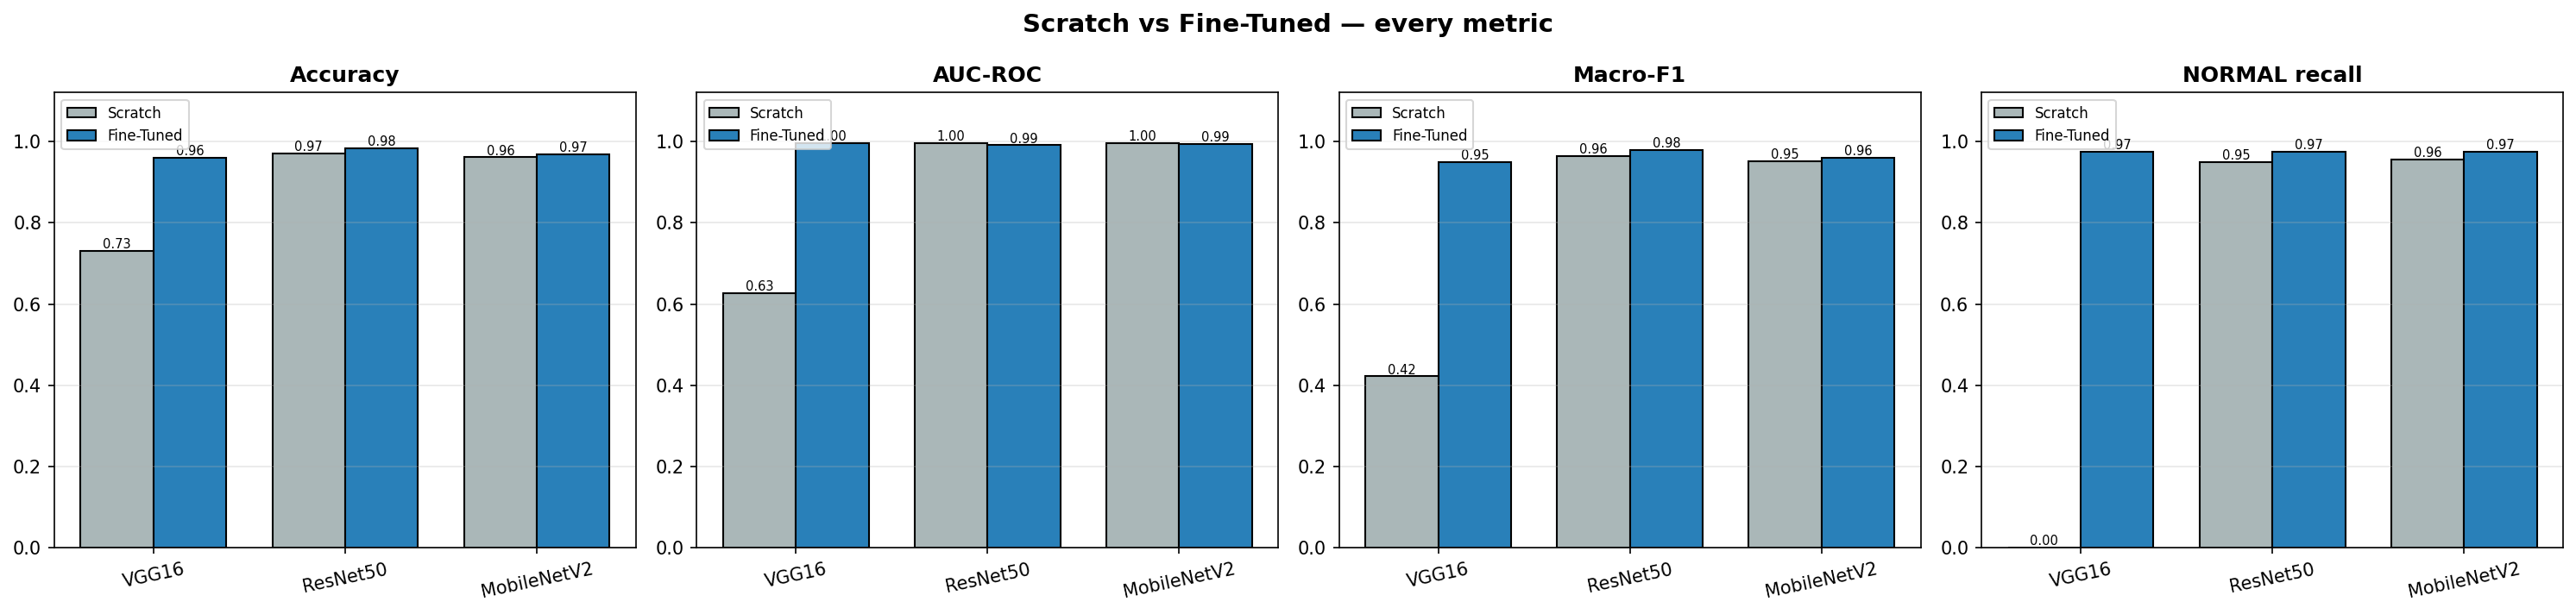
\includegraphics[width=0.85\textwidth]{p3_scratch_vs_finetuned.png}
\caption{From-scratch versus fine-tuned, every metric and architecture.}
\label{fig:8}
\end{figure}

In Figure~\ref{fig:8} the VGG16 panel is the dominant effect: a non-functional model becomes a strong
detector after fine-tuning. ResNet50 and MobileNetV2 show smaller but consistent gains in accuracy,
macro-F1, and minority recall, with AUC effectively tied near the ceiling.

\begin{figure}[H]
\centering
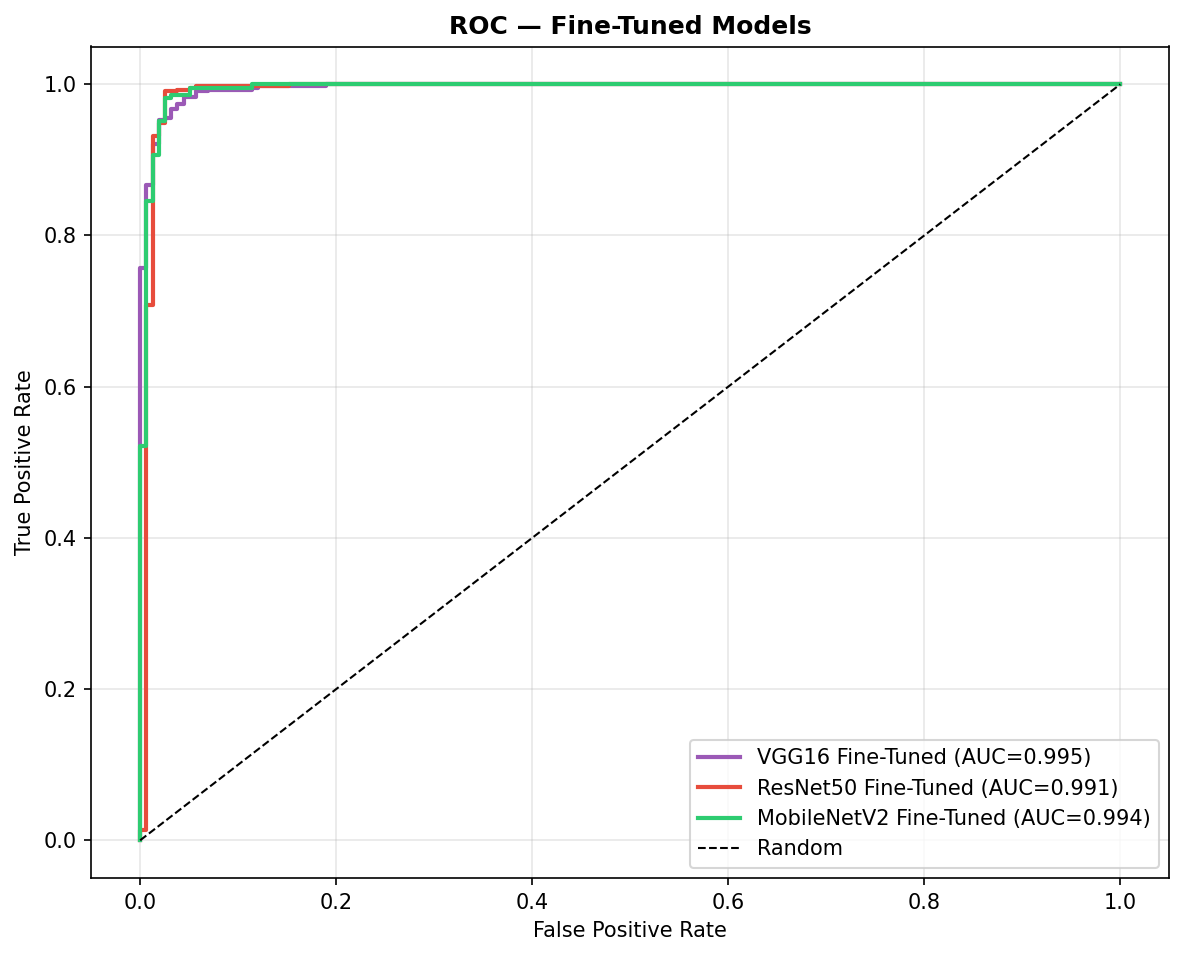
\includegraphics[width=0.7\textwidth]{p3_roc_finetuned.png}
\caption{ROC curves of the three fine-tuned models.}
\label{fig:9}
\end{figure}

In Figure~\ref{fig:9} all three fine-tuned models approach AUC $\approx0.99$.

\subsection{Training dynamics and confusion matrix of the best model}

\begin{figure}[H]
\centering
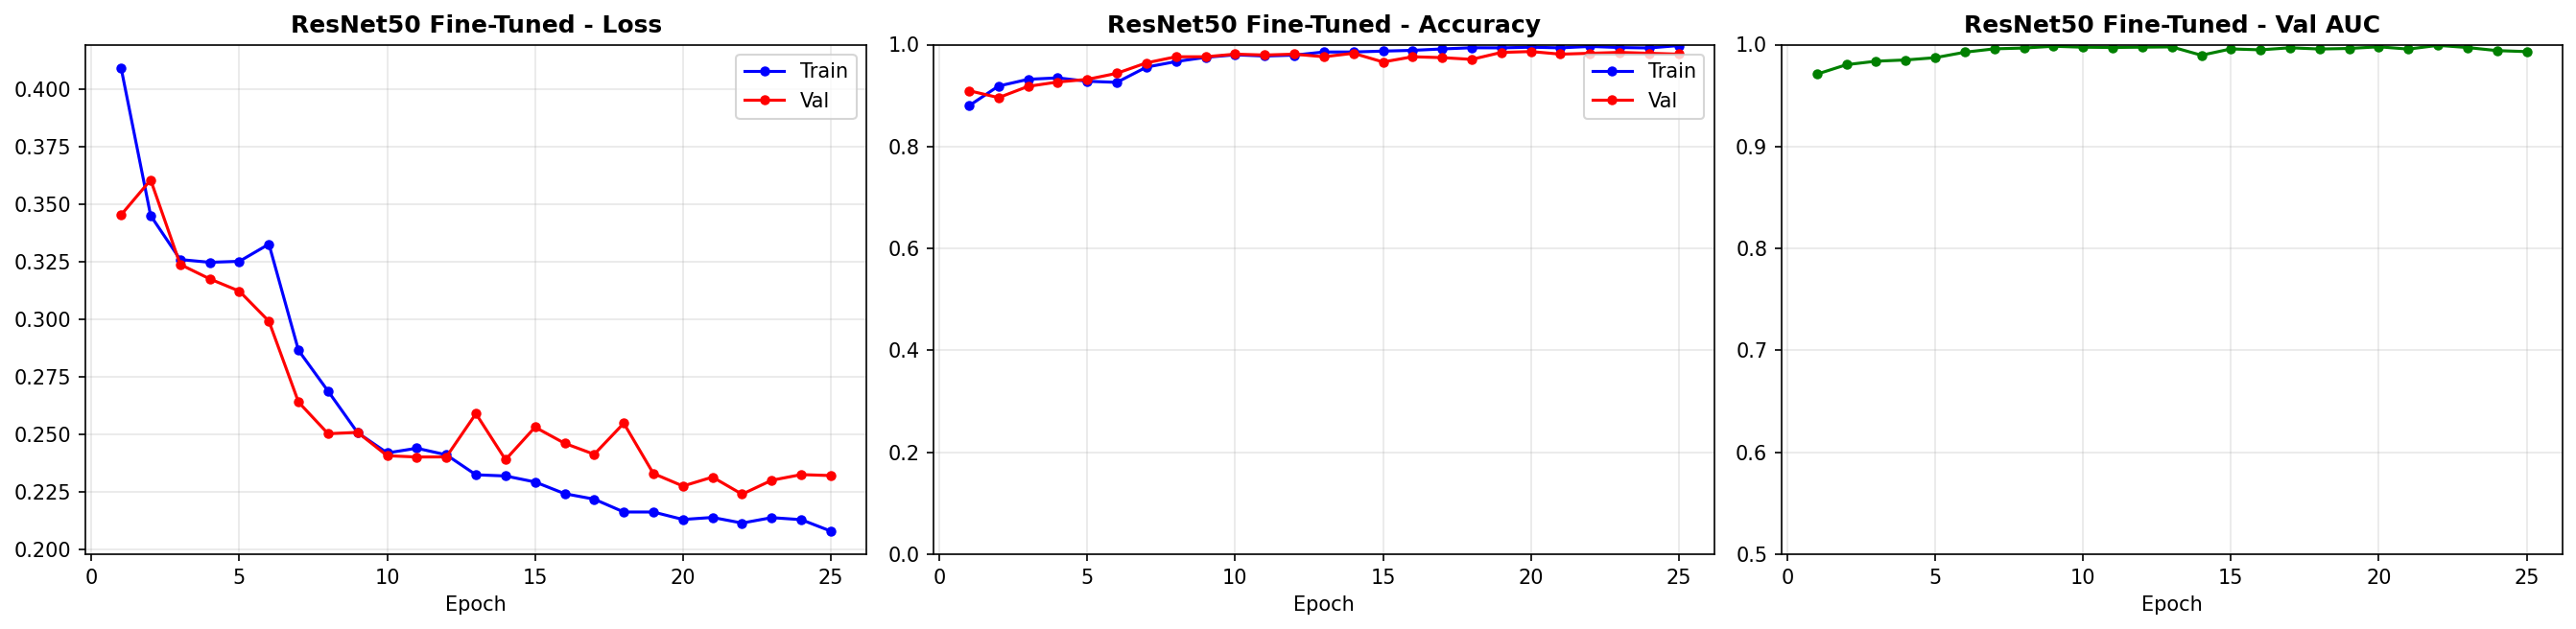
\includegraphics[width=0.85\textwidth]{resnet50_fine-tuned_curves.png}
\caption{Training curves of ResNet50 fine-tuned across epochs.}
\label{fig:10}
\end{figure}

In Figure~\ref{fig:10}, the discontinuity at the Phase~1$\rightarrow$Phase~2 boundary (epoch 5)
corresponds to backbone unfreezing, after which validation accuracy rises toward 0.98.

\begin{figure}[H]
\centering
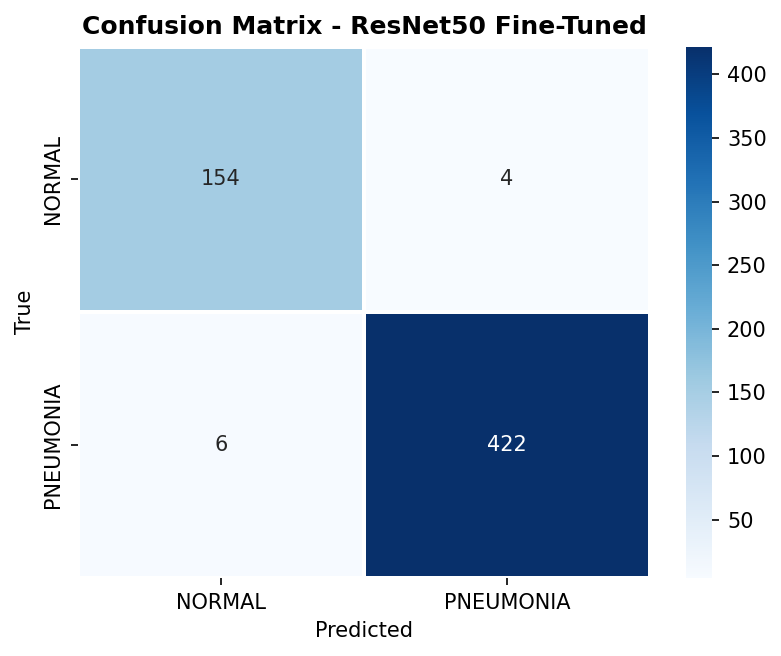
\includegraphics[width=0.6\textwidth]{resnet50_fine-tuned_cm.png}
\caption{Confusion matrix of ResNet50 fine-tuned (586-image test set).}
\label{fig:11}
\end{figure}

In Figure~\ref{fig:11} (rows = true, columns = predicted) the clinically critical false-negative
cell true PNEUMONIA predicted NORMAL is minimal: of the 428 true-PNEUMONIA cases the fine-tuned
ResNet50 misses only about six (PNEUMONIA recall 0.986), consistent with the asymmetric clinical cost
identified in Section~1.1, under which a missed pneumonia is the most damaging error.

\subsection{Interpretability of the best model (ResNet50 fine-tuned)}
Three complementary attribution methods were applied to a balanced set of six test images (three NORMAL,
three PNEUMONIA).

\begin{figure}[H]
\centering
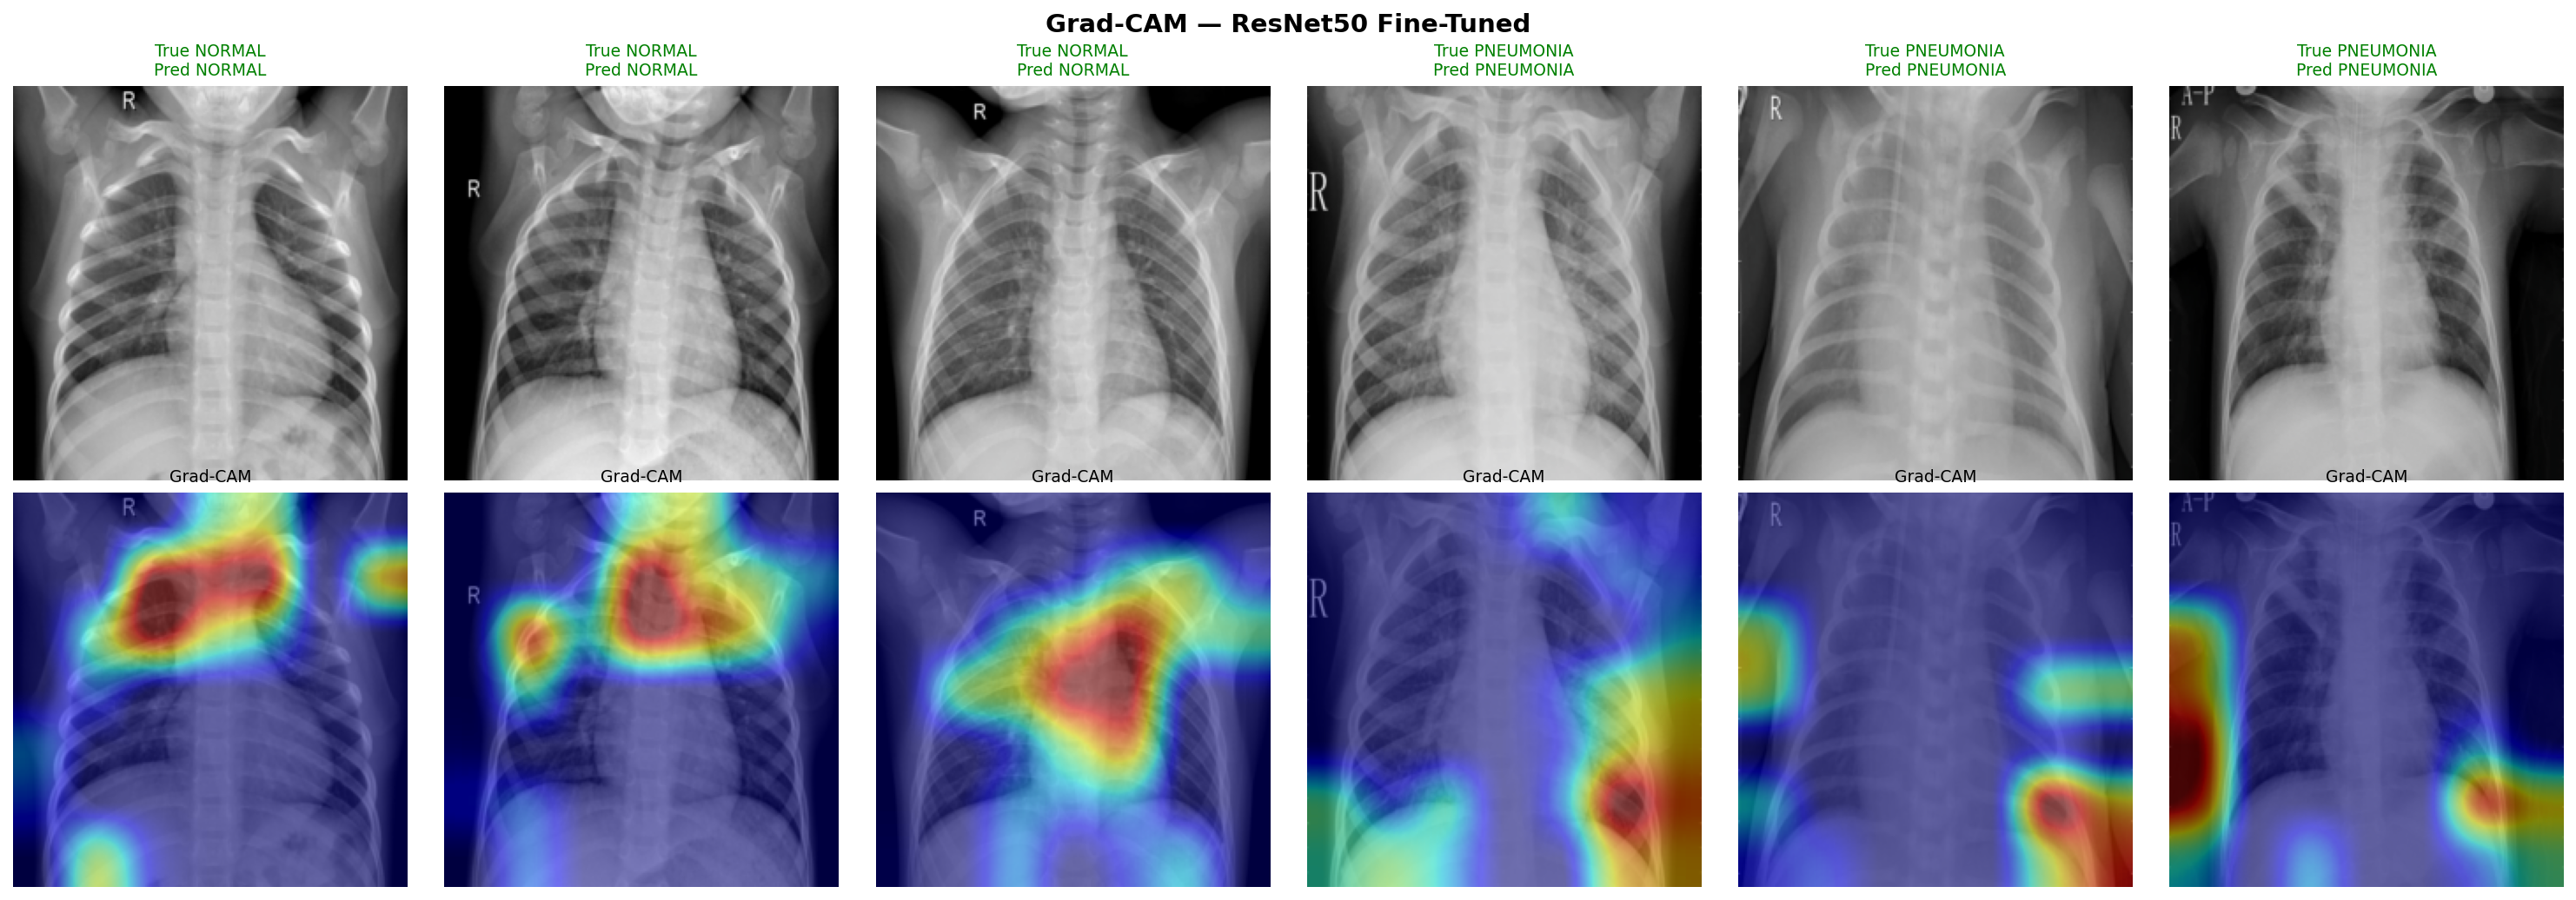
\includegraphics[width=0.85\textwidth]{p3_gradcam.png}
\caption{Grad-CAM heatmaps at the final convolutional layer.}
\label{fig:12}
\end{figure}

In Figure~\ref{fig:12}, warm regions indicate high attribution; for pneumonia cases the activation
concentrates on pulmonary opacities, and titles are coloured green where the prediction matches the
ground truth. The model attends to clinically relevant anatomy rather than borders or text markers.

\begin{figure}[H]
\centering
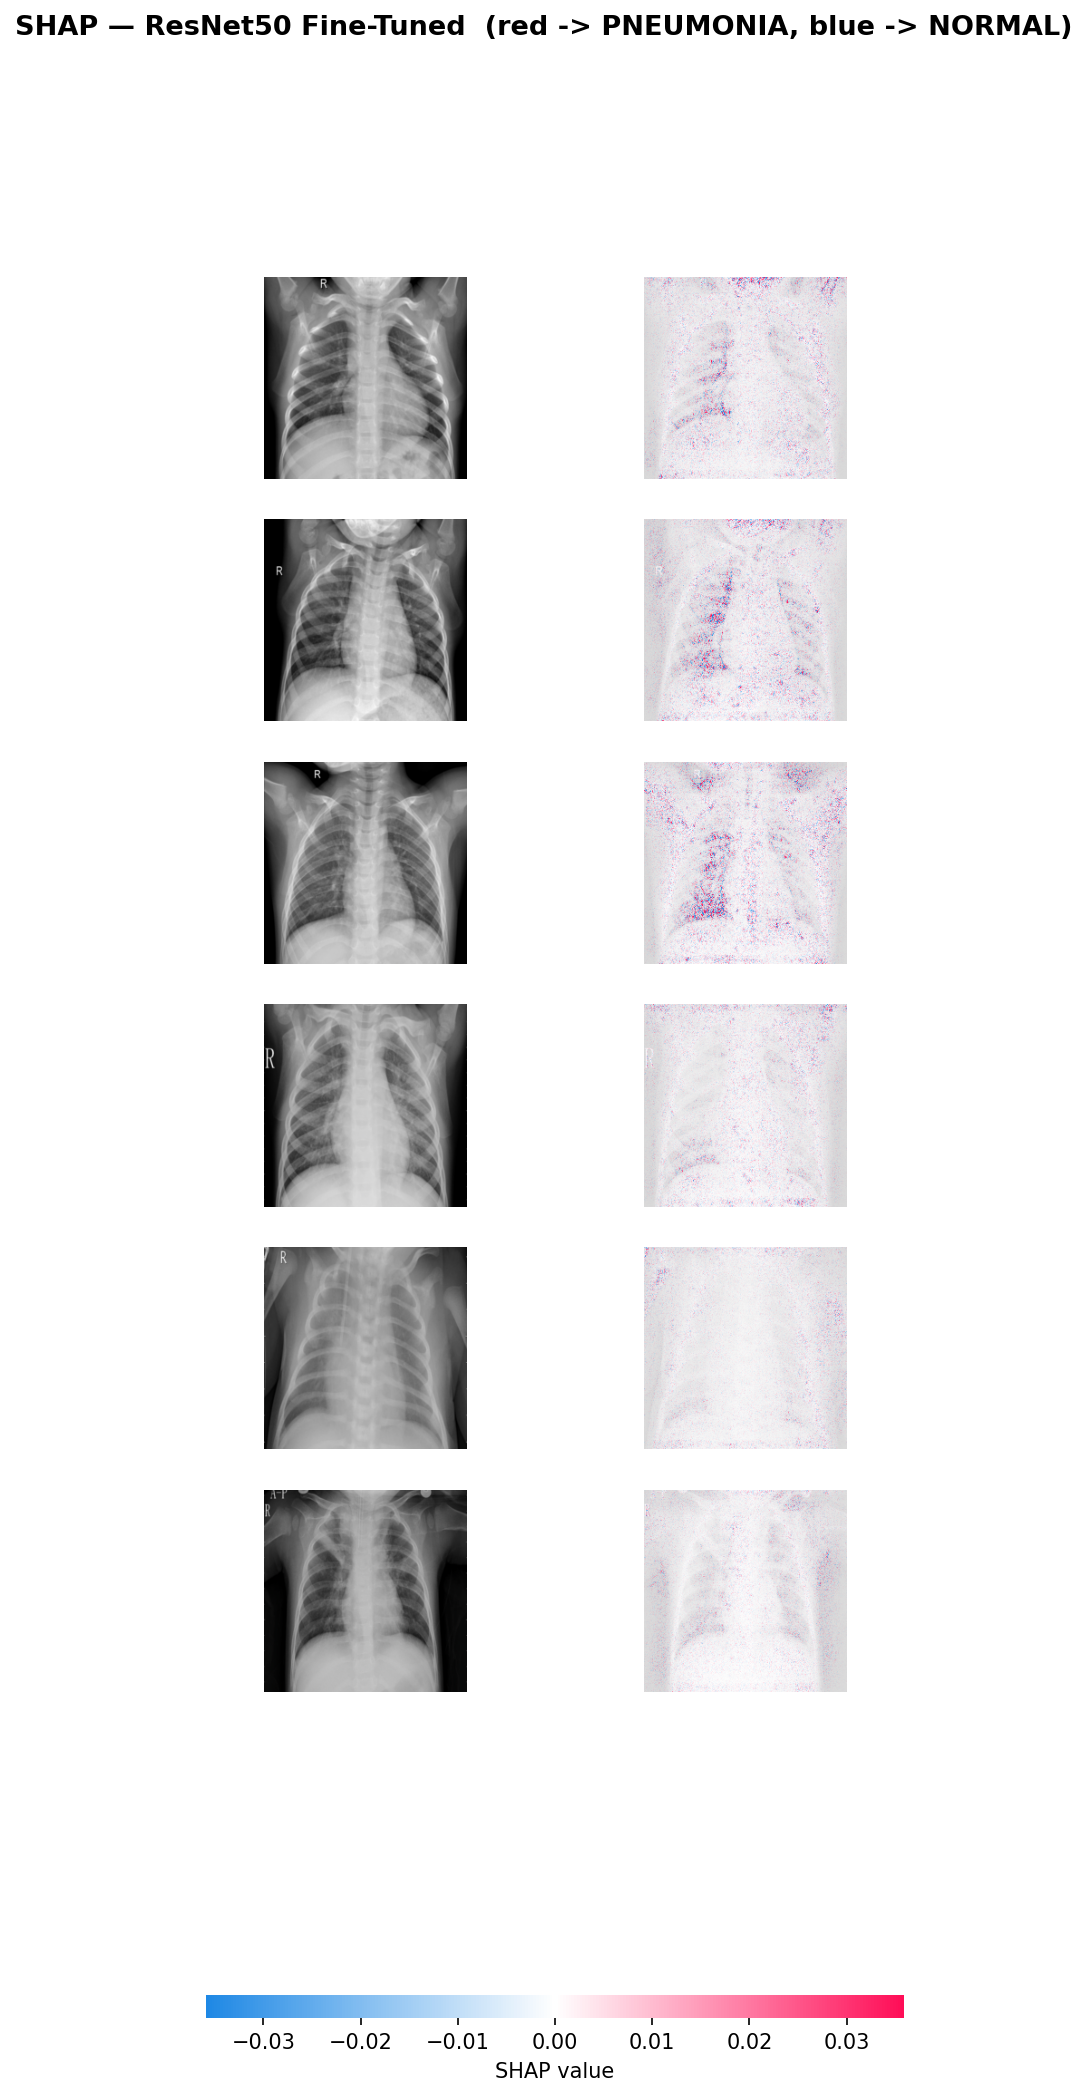
\includegraphics[width=0.7\textwidth]{p3_shap.png}
\caption{SHAP pixel attributions toward the PNEUMONIA class.}
\label{fig:13}
\end{figure}

In Figure~\ref{fig:13} (GradientExplainer) red pixels push the prediction toward PNEUMONIA and blue
toward NORMAL, providing a finer-grained view that is consistent with the Grad-CAM evidence.

\begin{figure}[H]
\centering
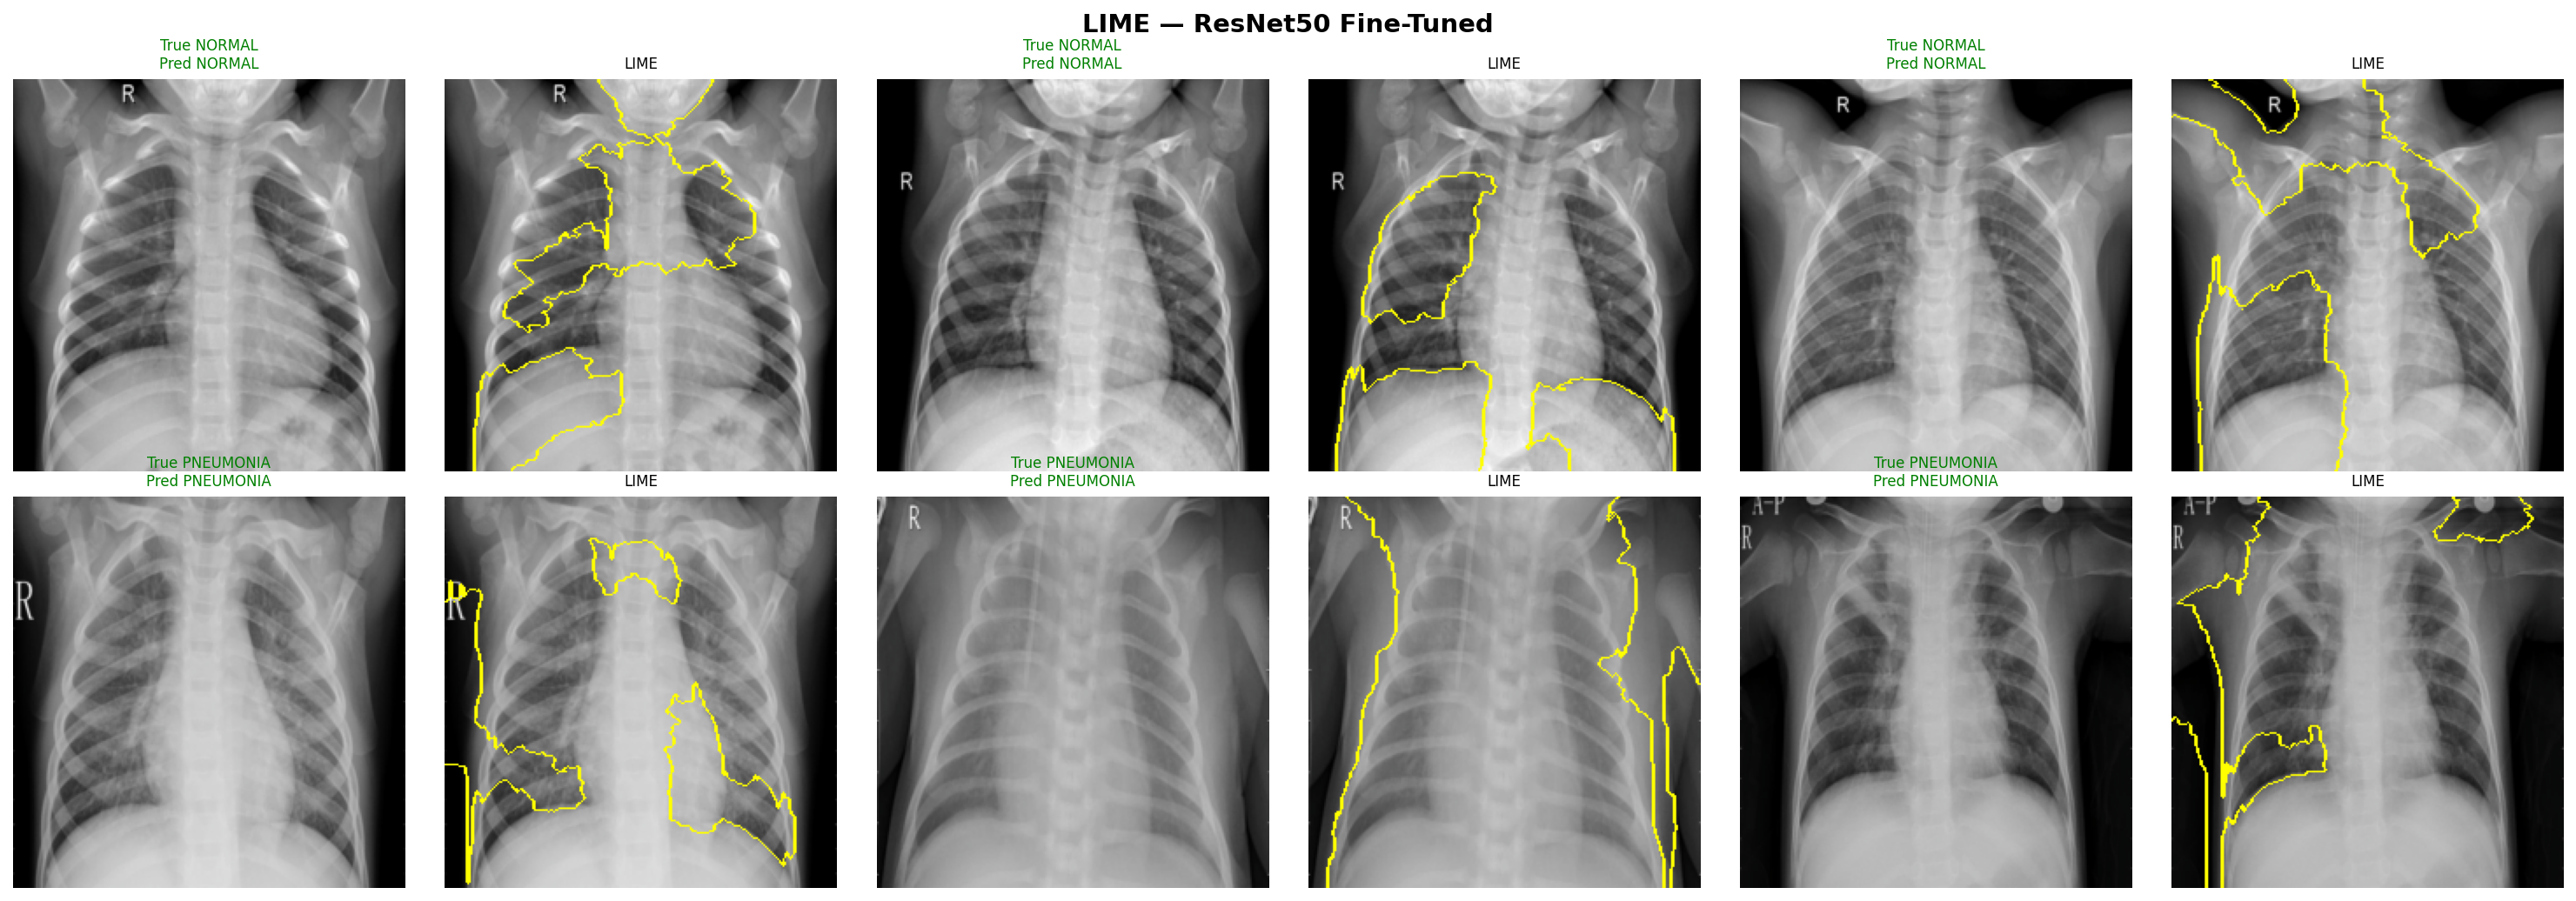
\includegraphics[width=0.85\textwidth]{p3_lime.png}
\caption{LIME explanations (1{,}000 perturbations, top-five superpixels).}
\label{fig:14}
\end{figure}

In Figure~\ref{fig:14} a third, model-agnostic method converges on the same lung regions, strengthening
the conclusion that the model relies on genuine pathological features rather than spurious correlations.

% ===================================================================
\section{Discussion}

% \subsection{What worked}
Correcting the data pipeline resolved the minority-class collapse observed in Experiment~1. After
stratified re-splitting and weighted sampling, NORMAL recall rose from 0.71 (Experiment~1) to 0.95 for
the BatchNorm-equipped from-scratch models (ResNet50 0.9494, MobileNetV2 0.9557) and to 0.97 once those
backbones were fine-tuned, without sacrificing overall accuracy. Crucially, the clinically critical
metric PNEUMONIA recall, since a missed pneumonia is the costliest error (Section~1.1) also stayed
high throughout (0.986 for the best model): the imbalance correction raised minority (NORMAL) recall
without trading away sensitivity to disease. The most consequential result is the rehabilitation of
VGG16: a model that was entirely non-functional from scratch under our shared training recipe (0.00
minority recall) improved on every metric after fine-tuning ($+0.23$ accuracy, $+0.37$ AUC, $+0.97$
minority recall), the clearest demonstration in this study of transfer learning's value. Matching the
fine-tuning recipe to each architecture a gentle partial unfreeze with gradient clipping for VGG16, and
a full unfreeze for the BatchNorm-stabilised networks was necessary to move every metric in the
intended direction. The best model, ResNet50 fine-tuned, reached 0.9829 accuracy and 0.9784 macro-F1.\\

% \subsection{What did not improve as expected}
AUC-ROC did not strictly increase for the two already-strong backbones: ResNet50 ($-0.0056$) and
MobileNetV2 ($-0.0011$) recorded marginally lower AUC after fine-tuning. Because their from-scratch AUC
was already $\approx0.996$ effectively at the measurement ceiling for a 586-image test set these
sub-0.6\% differences are most plausibly noise rather than genuine regression. This remains an
interpretation rather than a demonstrated result: with a single seed per configuration
(Section~\ref{sec:limits}) no variance can be estimated, so the claim is offered as the most parsimonious
reading of a near-ceiling difference, not as a statistically supported one. Where the baseline is already
near-perfect, the available headroom lies in the operating-point metrics (accuracy, macro-F1, minority
recall), which is where the measurable gains occurred. A second negative result is methodological: a
single full-unfreeze recipe would likely have destabilised VGG16, so the per-architecture treatment was a
requirement, not a refinement.\\

% \subsection{Interpretation}
The balanced training set (4{,}684 images) is large enough, and the task sufficiently separable
(consolidation is a strong visual signal), that BatchNorm-equipped networks converge well even from
scratch. This compresses the transfer-learning margin for ResNet50 and MobileNetV2 to ``modest but
consistent.'' The margin becomes decisive only where from-scratch optimisation fails outright (VGG16),
supporting the general observation that the benefit of pretraining scales with the difficulty of the
from-scratch problem.\\

% \subsection{Limitations}
\label{sec:limits}
Several limitations qualify these results. Each experiment uses a single train/validation/test split and
a single random seed, so no confidence intervals are available and small differences particularly the
near-ceiling AUC gaps are not subjected to statistical testing. The dataset is also pediatric and drawn
from a single source, which means the findings may not transfer to adult cohorts or to multi-institution
radiographs acquired under different protocols. The task itself is restricted to a binary
NORMAL-versus-PNEUMONIA decision, whereas clinical triage typically involves multiple co-occurring
findings and explicit measures of uncertainty. Finally, the stratified re-splitting that was necessary to
obtain a reliable validation set precludes direct numerical comparison with prior work that reports on
the original Kaggle partition. For context, the dataset's originators \cite{kermany} reported roughly
92.8\% accuracy on the official split; our 98.3\% is measured on a different, stratified test partition
and is therefore not directly comparable, and should not be read as a state-of-the-art claim.\\

% \subsection{Threats to validity}
\label{sec:threats}
The scratch-versus-fine-tune comparison is not a perfectly isolated A/B test of pretraining. Two
confounds qualify the deltas in Table~\ref{tab:delta}. (i) \textbf{Test-time augmentation:} the
fine-tuned models are evaluated with TTA (averaging the original and horizontally-flipped predictions),
whereas the from-scratch models are evaluated without it; a fraction of the fine-tuned advantage may
therefore be attributable to TTA rather than to pretraining. (ii) \textbf{Training-protocol
differences:} the fine-tuning path also adds label smoothing and a two-phase discriminative-rate schedule
absent from the scratch path. These auxiliary factors are small relative to the headline VGG16 effect (a
0.97 swing in minority recall cannot be explained by a flip-averaging trick), but they mean the modest
ResNet50 and MobileNetV2 gains should be read as the effect of the \emph{complete transfer-learning
protocol}. A cleaner future design would apply identical evaluation (TTA on or off for both arms) and
identical loss and schedule to both arms, leaving initialisation as the only difference.

% ===================================================================
\section{Conclusion}
This report demonstrated, through three controlled experiments, that (i) class imbalance can silently
destroy minority-class recall and must be handled explicitly a \texttt{WeightedRandomSampler} achieved
this and (ii) ImageNet transfer learning, applied through an architecture-aware two-phase fine-tuning
procedure, improves pneumonia detection relative to training from scratch. The improvement ranged from
modest-but-consistent for already-strong backbones (ResNet50, MobileNetV2) to decisive for a backbone
that did not train from scratch under our shared, architecture-agnostic recipe (VGG16, 0.00 $\rightarrow$
0.97 minority recall). The best configuration, ResNet50 fine-tuned, achieved 0.9829 accuracy and 0.9784
macro-F1, and three independent attribution methods confirmed that it bases its decisions on clinically
relevant lung regions.\\

Per-class recall and AUC-ROC must be reported alongside accuracy, since
accuracy alone masked a 30\% minority-miss rate. Transfer learning helps most precisely where
from-scratch training fails, and its measurable gains shrink with AUC effectively tied once the
from-scratch baseline approaches the ceiling. Reliable fine-tuning depends on BatchNorm-statistic
freezing, discriminative learning rates, and an unfreezing scope matched to the architecture.\\

Natural extensions include k-fold cross-validation with multiple seeds and
significance testing; evaluation of newer backbones (DenseNet121, EfficientNet) and external datasets
(CheXpert, NIH) for cross-domain validation; decision-threshold calibration to optimise clinical
sensitivity, and focal loss as an alternative imbalance strategy; and a multi-label extension to detect
co-occurring pathologies.

% ===================================================================
\clearpage
\phantomsection
\addcontentsline{toc}{section}{References}
% ===================================================================
\begin{thebibliography}{10}
\bibitem{kermany} D.~S. Kermany \textit{et al.}, ``Identifying medical diagnoses and treatable diseases by image-based deep learning,'' \textit{Cell}, vol.~172, no.~5, pp.~1122--1131.e9, Feb.\ 2018, doi: 10.1016/j.cell.2018.02.010.
\bibitem{resnet} K.~He, X.~Zhang, S.~Ren, and J.~Sun, ``Deep residual learning for image recognition,'' in \textit{Proc.\ IEEE CVPR}, 2016, pp.~770--778, doi: 10.1109/CVPR.2016.90.
\bibitem{vgg} K.~Simonyan and A.~Zisserman, ``Very deep convolutional networks for large-scale image recognition,'' in \textit{Proc.\ ICLR}, 2015. arXiv:1409.1556.
\bibitem{mobilenet} M.~Sandler, A.~Howard, M.~Zhu, A.~Zhmoginov, and L.-C. Chen, ``MobileNetV2: Inverted residuals and linear bottlenecks,'' in \textit{Proc.\ IEEE/CVF CVPR}, 2018, pp.~4510--4520, doi: 10.1109/CVPR.2018.00474.
\bibitem{imagenet} J.~Deng, W.~Dong, R.~Socher, L.-J. Li, K.~Li, and L.~Fei-Fei, ``ImageNet: A large-scale hierarchical image database,'' in \textit{Proc.\ IEEE CVPR}, 2009, pp.~248--255, doi: 10.1109/CVPR.2009.5206848.
\bibitem{gradcam} R.~R. Selvaraju, M.~Cogswell, A.~Das, R.~Vedantam, D.~Parikh, and D.~Batra, ``Grad-CAM: Visual explanations from deep networks via gradient-based localization,'' in \textit{Proc.\ IEEE ICCV}, 2017, pp.~618--626, doi: 10.1109/ICCV.2017.74.
\bibitem{shap} S.~M. Lundberg and S.-I. Lee, ``A unified approach to interpreting model predictions,'' in \textit{Proc.\ NeurIPS}, vol.~30, 2017.
\bibitem{lime} M.~T. Ribeiro, S.~Singh, and C.~Guestrin, ```Why should I trust you?': Explaining the predictions of any classifier,'' in \textit{Proc.\ 22nd ACM SIGKDD}, 2016, pp.~1135--1144, doi: 10.1145/2939672.2939778.
\bibitem{pytorch} A.~Paszke \textit{et al.}, ``PyTorch: An imperative style, high-performance deep learning library,'' in \textit{Proc.\ NeurIPS}, vol.~32, 2019, pp.~8024--8035.
\bibitem{batchnorm} S.~Ioffe and C.~Szegedy, ``Batch normalization: Accelerating deep network training by reducing internal covariate shift,'' in \textit{Proc.\ 32nd ICML}, 2015, pp.~448--456.
\end{thebibliography}
% ===================================================================
\appendix
\section{Mapping to Assignment Requirements}
\begin{table}[H]
\centering
\caption{Requirement coverage.}
\label{tab:appA}
\begin{tabularx}{\textwidth}{XXl}
\toprule
Requirement & How addressed & Evidence \\
\midrule
Fine-tune a pretrained CNN on a medical dataset & VGG16 / ResNet50 / MobileNetV2 fine-tuned (ImageNet $\rightarrow$ X-ray), two-phase procedure & \S3.4; Table~\ref{tab:exp3} \\
Compare scratch versus fine-tuning on the same dataset & Identical balanced split, sampler, and evaluation; per-metric change table & Tables~\ref{tab:exp2}--\ref{tab:delta}; Figs.~\ref{fig:6}--\ref{fig:8} \\
Apply class-weighted loss or oversampling & Oversampling via \texttt{WeightedRandomSampler} (inverse-frequency) & \S3.3; Figs.~\ref{fig:3}--\ref{fig:4} \\
Report AUC-ROC in addition to accuracy & Both reported for every model; ROC curves provided & Tables~\ref{tab:exp1}--\ref{tab:exp3}; Figs.~\ref{fig:5},\ref{fig:7},\ref{fig:9} \\
Visualise what the network learns (Grad-CAM or similar) & Grad-CAM, SHAP, and LIME applied to the best model & Figs.~\ref{fig:12}--\ref{fig:14} \\
\bottomrule
\end{tabularx}
\end{table}
All five requirements are met; the visualisation requirement is exceeded through three independent
methods.

\section{Figure-to-File Index}
\begin{table}[H]
\centering
\caption{Figure-to-file index.}
\label{tab:appB}
\begin{tabular}{cll}
\toprule
Figure & File & Section \\
\midrule
2.1 & results2/p2\_class\_distribution.png & 2.3 \\
2.2 & results1/p1\_sample\_images.png & 2.3 \\
2.3 & results2/p2\_sampled\_batch.png & 2.3 \\
4.1 & results1/p1\_per\_class\_recall.png & 4.1 \\
4.2 & results1/p1\_roc\_curves.png & 4.1 \\
4.3 & results2/p2\_metric\_comparison.png & 4.2 \\
4.4 & results2/p2\_roc\_curves.png & 4.2 \\
4.5 & results3/p3\_scratch\_vs\_finetuned.png & 4.3 \\
4.6 & results3/p3\_roc\_finetuned.png & 4.3 \\
4.7 & results3/resnet50\_fine-tuned\_curves.png & 4.4 \\
4.8 & results3/resnet50\_fine-tuned\_cm.png & 4.4 \\
4.9 & results3/p3\_gradcam.png & 4.5 \\
4.10 & results3/p3\_shap.png & 4.5 \\
4.11 & results3/p3\_lime.png & 4.5 \\
\bottomrule
\end{tabular}
\end{table}
Per-model training curves and confusion matrices for the remaining experiments are available in
\texttt{results1/}, \texttt{results2/}, and \texttt{results3/}.

\vspace{1.0cm}
\begin{center}
{\small Code, notebooks, and all result figures:
\textcolor{blue}{\url{https://github.com/spaul571/Transfer-Learning-for-Medical-Imaging}}\par}
\end{center}



\end{document}
